\documentclass[journal, onecolumn]{IEEEtran}
\IEEEoverridecommandlockouts


% En caso de requerir agregar algún paquete, favor de ponerlo en el archivo
% "paquetes.tex". Ahí ya están algunos, los más comunes para importar imágenes, 
% ecuaciones, símbolos e importar código. Según yo son los necesarios para hacer
% el reporte. Pero de igual forma verificar y agregar según conveniencia. 
\usepackage[spanish]{babel}
\usepackage[utf8]{inputenc}
\usepackage{cite}
\usepackage{amsmath,amssymb,amsfonts}
\usepackage{algorithmic}
\usepackage{graphicx}
\usepackage{textcomp}
\usepackage{xcolor}
\usepackage{fancyhdr}
\usepackage{listings}
\usepackage{float}
\usepackage{blindtext}
\usepackage{newtxmath}
\usepackage{wrapfig}
\usepackage{mathtools}
\usepackage{breqn}
\usepackage{titlesec}
\usepackage{multirow}

\usepackage[flushleft]{threeparttable}
\usepackage{makecell,booktabs}

\usepackage[hyphens]{url}
\usepackage[hidelinks]{hyperref}


\lstdefinestyle{code}{%
backgroundcolor=\color{gray!1},
basicstyle=\ttfamily\small,
commentstyle=\color{green!60!black},
keywordstyle=\color{magenta},
stringstyle=\color{blue!50!red},
showstringspaces=false,
%captionpos=b,
numbers=left,
numberstyle=\footnotesize\color{gray},
numbersep=5pt,
%stepnumber=2,
tabsize=2,
%frame=L,
%framerule=1pt,
%rulecolor=\color{red},
breaklines=true,
}
\decimalpoint
\hypersetup{breaklinks=true}


\titlespacing*{\section}
{0pt}{2.0ex plus 1ex minus .2ex}{1.0ex plus .2ex}
\titlespacing*{\subsection}
{0pt}{2.0ex plus 1ex minus .2ex}{1.0ex plus .2ex}
\titlespacing*{\subsubsection}
{0pt}{2.0ex plus 1ex minus .2ex}{1.0ex plus .2ex}

\renewcommand\IEEEkeywordsname{Palabras Clave}


\def\BibTeX{{\rm B\kern-.05em{\sc i\kern-.025em b}\kern-.08em
    T\kern-.1667em\lower.7ex\hbox{E}\kern-.125emX}}


\graphicspath{ {../Imagenes/} }

\numberwithin{equation}{section}
\numberwithin{figure}{section}
\numberwithin{table}{section}

\newcommand{\scaleFigures}{0.5}
\renewcommand{\thesection}{\arabic{section}}
%\renewcommand{\thesubsection}{\arabic{subsection}}


\begin{document}
    \renewcommand{\tablename}{Tabla}
    \bstctlcite{IEEEexample:BSTcontrol}
    \title{Métodos para súper-resolución de imágenes}
    
    \author{\IEEEauthorblockN{Madrigal-Custodio Jesús A., Tevera-Ruiz Alejandro, Torres-Martínez Luis Á.\\}
    \IEEEauthorblockA{\textit{Departamento: Robótica y Manufactura Avanzada} \\
    \textit{Centro de Investigación y de Estudios Avanzados del Instituto Politécnico Nacional}}
    }

    \maketitle

    \begin{abstract}
        En el presente documento se explican los fundamentos, metodología y proceso de implementación 
        para el desarrollo de algoritmos de súper resolución bajo diversos enfoques con el objetivo... 
    \end{abstract}

    \begin{IEEEkeywords}
    Súper Resolución, Redes Convolucionales, Inteligencia Artificial
    \end{IEEEkeywords}

    \section{Introducción}
    % Comando para importar archivos en la plantilla.
    % Para ello deberá crear el archivo .tex en la carpeta "Secciones" 
    % Y posteriormente importarlo con el comando "input".

    % Cada que realice un cambio en el main favor de actualizarlo en el 
    % repo para no tener problemas en el manejo de este archivo que todos
    % moveremos. Lo mismo para el archivo paquetes.
    
    % Para el resto no es necesario. 


    
El gran reto de estimar una imagen de alta resolución, teniendo de base una imagen de baja calidad es a lo que se le conoce como 
\emph{Super Resolución},la Super-Resolución para una sola imagen (SISR) es un problema que ha sido estudiado desde antes del siglo XXI, lo que comenzó tiempo atrás
como un tema de ciencia ficción termino por ser un tema de investigación que aun no culmina, pero presenta avances significativos en la actualidad.
Existen muchos antecedentes sobre modelos que tratan de recuperar la información de las imágenes de baja resolución haciendo un escalado de esta y 
 con el uso de modelos probabilísticos estimar los datos faltantes, otros que aplican parches en combinación con imágenes de alta resolución para lograr un 
 resultado legible sentando un precedente en la investigación.
 
 A pesar de estos esfuerzos aun se buscaba mejorar estas estimaciones, con el surgimiento de las \emph{Redes Neuronales Artificiales}, capaces de realizar predicciones dada sus
habilidad de aprendizajes, podían obtener modelos precisos de una tarea especifica a partir de fragmentos de información con los cuales realizan un entrenamiento. De
esta nueva estrategia surgen entonces diferentes modelos de redes Neuronales como los son las Convolucionales, GAN´s, Residuales, entre otras.Esto 
se puede considerar hasta ahora el mayor avance en cuanto a super resolución.

El objetivo de este trabajo es realizar una comparativa entre 3 diferentes métodos para la obtención de Super Resolución, se consideran el algoritmo de Freeman \cite{freeman},
la Super resolución por Redes Neuronales Convolucionales \cite{SRCNN} y las Redes Generativas Adversarias \cite{SRGAN}. Al aplicar estos modelos se busca
visualizar claramente como se estructura cada uno, cuales son las ventajas y desventajas, cuantificar el avance tecnológico y dar un panorama sobre lo alcanzado en la actualidad
mediante la comparativa de resultados. 
    \subsection{SRGAN}
Las GANs presentan varios desafíos a eludir durante su entrenamiento
que son actualmente temas de investigación. Entre ellos, los problemas más
usuales que surgen en el entrenamiento de una GAN son:

No convergencia
El generador y el discriminador no logran alcanzar un equilibrio. La
función de pérdida del generador y discriminador empiezan a oscilar sin
poder lograr a largo plazo una estabilidad.
Si bien es común en las GAN que en un comienzo las funciones de pérdida
oscilen, a medida que transcurre el entrenamiento el objetivo es que se
logre una estabilidad. Cuando esto no ocurre, las muestras son producidas
por el generador, pero su calidad no mejora.
Colapso modal
Esto ocurre cuando el generador produce muestras similares aunque las
entradas sean de muy diversas características. El generador encuentra que
un conjunto pequeño de muestras engañan al discriminador y entonces
no es capaz de producir otras. En estos casos, el gradiente de la función
de pérdida queda estancado en un valor cercano a 0.
Pérdida no informativa
Aunque parezca natural pensar que cuanto menor sea la pérdida del
generador, mayor será la calidad de las muestras que produce, esto no
resulta tan inmediato. La pérdida del generador debe ser comparada con
la del discriminador, que se encuentra en constante mejora. Por lo tanto,
no es tan sencillo evaluar la mejora del modelo. El generador podría estar
produciendo muestras cada vez de mayor calidad, aun cuando la función
de pérdida se vaya incrementando.


Pérdida del Generador -- max: 228.5551261019351, min: 23.898190839255033
Pérdida Discriminador -- max: 1.236285184701566, min: 1.6890162633455543e-16
Precisión Discriminador -- max: 1.0, min: 0.8630597014925373


    \section{Antecedentes}
    % Introducción a los tres enfoques y enfatizar el trabajo a mano por Freeman. 
\noindent
Bajo un enfoque \emph{clásico}, existen tres formas de mejorar la resolución 
de una imagen:

\begin{itemize}
    \item Amplificación de detalles existentes
    \item Suma de múltiples frames
    \item Único frame
\end{itemize}

Para el primero de ellos, se realiza una amplificación de las frecuencias altas
(donde se encuentran los detalles existentes de la imagen) dada la variación local
entre los pixeles vecinos. 
La amplificación de detalles existentes resulta bastante 
sencillo de aplicar. Sin embargo, ante imágenes con una cantidad considerable de
ruido puede no ser la mejor opción a tomar. Además, al potencializar las 
frecuencias ya existentes de la imagen, el resultado estará definido por el detalle
previo en la imagen de entrada. 

El segundo de los métodos considera que el frame de alta resolución es el resultado
de una secuencia de frames de baja resolución que permiten obtener las frecuencias 
altas de la imagen resultante para mejorar su resolución. Esto es conveniente cuando
ya se cuenta con el conjunto de imágenes requeridas y se planea realizar una 
reconstrucción de la imagen en una mejor calidad.

Por otro lado, el tercer método basado en un único frame o imagen busca aproximar las
frecuencias altas (detalles) que no se encuentra en la entrada del algoritmo y que evidentemente
no puede obtenerse sólo amplificando las frecuencias altas como lo que ocurre con 
el primero de los métodos. 

\subsubsection{Interpolación}
\noindent
Para mejorar la calidad se busca aumentar la densidad de pixeles de la imagen con el objetivo
de hacer la imagen más grande y mejorar sus detalles a partir de la predicción de 
pixeles que no se encuentran en la imagen visiblemente, pero que podrían aproximarse
al buscar que se mantenga una consistencia en la imagen modificada de acuerdo a la
vecindad de los pixeles. 

Esto permite proponer el uso de algoritmos de interpolación que buscan predecir los 
pixeles vecinos y con ello aumentar la densidad de pixeles de la imagen de entrada. 
Con base en \cite{interpolation_cambridge}, dichos algoritmos pueden agruparse en dos categorías: adaptativos y no adaptativos.
Los primeros cambian dependiendo de lo que se está interpolando (bordes o texturas 
suaves) pixel por pixel con el objetivo de minimizar los errores antiestéticos
de los algoritmos de interpolación como el desenfoque o pérdida de detalles en 
regiones evidentes. Ejemplos de ellos pueden ser los softwares de licencia como
\emph{Qimage, PhotoZoom Pro, Genuine Fractals, etc}. 

Mientras que los métodos no adaptativos tratan todos los pixeles por igual
dada la predicción de un pixel central de acuerdo a sus pixeles adyacentes. Esto 
involucra que entre más vecinos se consideren en la interpolación, una mejor 
aproximación se tendrá del pixel a predecir, pero de manera proporcional 
aumentarán los recursos computacionales necesarios. Dentro de los algoritmos 
se incluyen: \emph{vecino más cercano, bilineal, bicúbica, spline, entre otros.}

A continuación se describirán algunos de los algoritmos no adaptativos para 
interpolación que serán utilizados en los diferentes métodos para \emph{Súper
Resolución}:
\begin{itemize}
    \item \textbf{Vecino más cercano} - Dado un pixel considera sólo un pixel 
    adyacente para la interpolación, lo que resulta en un menor tiempo de procesamiento
    pero resultados poco consistentes al observar al conjunto de pixeles interpolados. 
    \item \textbf{Bilineal} - Considera una vecindad 2x2 correspondiente al pixel
    a predecir con su correspondiente promedio ponderado de acuerdo a la distancia
    del pixel desconocido. Esto da como resultado un aspecto más suave que el vecino
    más cercano. 
    \item \textbf{Bicúbica} - Valora una vecindad 4x4 de pixeles conocidos para la
    predicción del pixel central considerando el mismo procedimiento de la 
    interpolación bilineal. Como resultado, se alcanzan imágenes más nítidas que los 
    métodos anteriores. Logrando así un equilibrio entre la calidad de salida y el 
    tiempo de procesamiento. Lo anterior promueve que sea un estándar en muchos programas
    de edición de imágenes, controladores de impresoras e interpolación en cámaras. 
\end{itemize}


\textbf{NOTA: Agregar comparativo de interpolaciones con un parche y escalado x2}


    \subsection{Example Based Super Resolution}
\noindent
Como puede observarse la interpolación soluciona parcialmente el problema de
\emph{Súper Resolución}, pero tiene como consecuencia los efectos mencionados. En
particular, el desenfoque resulta contraproducente al intentar mejorar los 
detalles de una imagen. Por lo mismo, en los algoritmos clásicos de \emph{Súper Resolución}
se utiliza la interpolación únicamente para aumentar la densidad de los pixeles
y aproximar la imagen de salida como una imagen más grande con un determinado 
factor de escalado, pero con los detalles de desenfoque que producen los 
algoritmos de interpolación no adaptativos. 

Para solucionarlo, algunos autores proponen realizar un postprocesado a la imagen 
interpolada para incluir los detalles faltantes y con ello mejorar visiblemente 
la resolución de los bordes de la imagen. 

En particular, \cite{freeman} propone un parchado de la imagen reescalada a partir
de un conjunto de entrenamiento o diccionario de parches en pares de alta
y baja resolución. Dichos parches permiten construir una imagen con frecuencias
altas que no están en la imagen de entrada con el objetivo de sumar la imagen
original interpolada con las frecuencias altas que buscan mejorar su resolución
al realzar sus detalles. En la Figura \ref{fig:fr_algoritmo} puede observarse de
manera específica el algoritmo propuesto basado en el parchado de la imagen de 
entrada mediante un algoritmo de predicción.

\begin{figure}[H]
    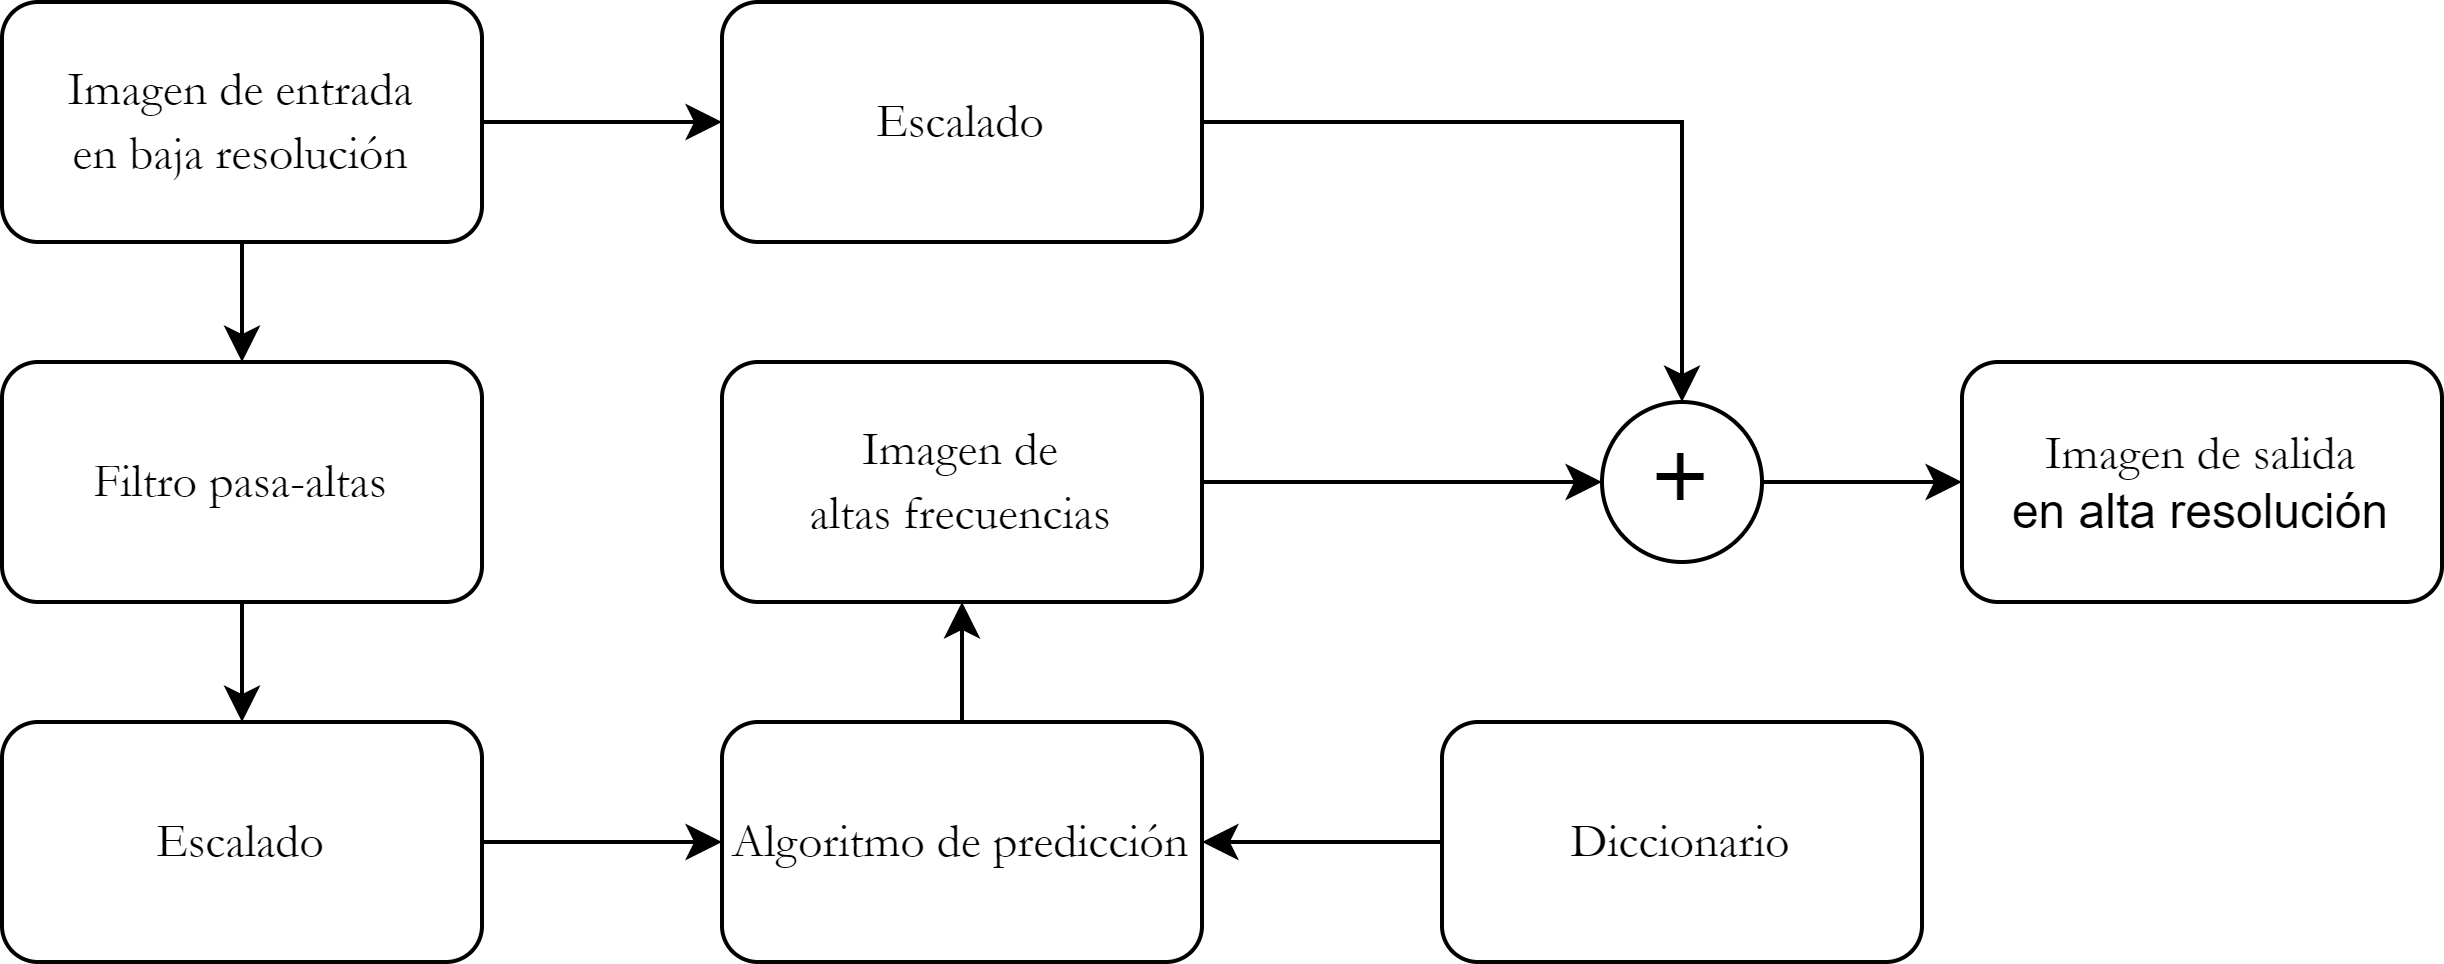
\includegraphics[scale = 0.5]{ fr_algoritmo.png }
    \centering
    \caption{ Algoritmo de súper resolución }
    \label{fig:fr_algoritmo}
\end{figure}

\subsubsection{Diccionario}
\noindent
El algoritmo de \emph{Súper Resolución} \cite{freeman}
opera bajo la premisa que la relación
de predicción entre los parches de alta y baja resolución es independiente del 
contraste de la imagen. Esto también resulta ventajoso, ya que el diccionario 
no necesita ser de imágenes similares a las que se van a reconstruir para 
mejorar la calidad de resolución tal como comenta \cite{diccionario_shuji}.
Esto resulta en un algoritmo general aplicable a cualquier tipo de imagen
y escalable respecto al tamaño de la base de entrenamiento.

Desde el punto de vista de almacenamiento, los parches de baja resolución carecen 
de detalle y por lo tanto predominan las frecuencias bajas, las cuales son 
irrelevantes en su uso para la predicción de detalles y por lo tanto resulta
información necesaria dentro del proceso. Por lo mismo, es aconsejable aplicar un filtro pasa-altas a cada parche 
con el objetivo de dejar sólo la información útil para el algoritmo (detalles).

Por otra parte, para que el diccionario sea funcional sin importar el 
tipo de imagen a reconstruir, se busca normalizar cada pareja de parche con el 
objetivo de mantener su relación intrínseca. De acuerdo con \cite{freeman}, 
los parches de baja resolución se recomiendan con un tamaño de 7x7 pixeles
mientras que los de alta resolución serán de 5x5 todos con centro en el mismo pixel
para mantener la relación tal como se presenta en la Figura \ref{fig:fr_dic}.

\begin{figure}[H]
    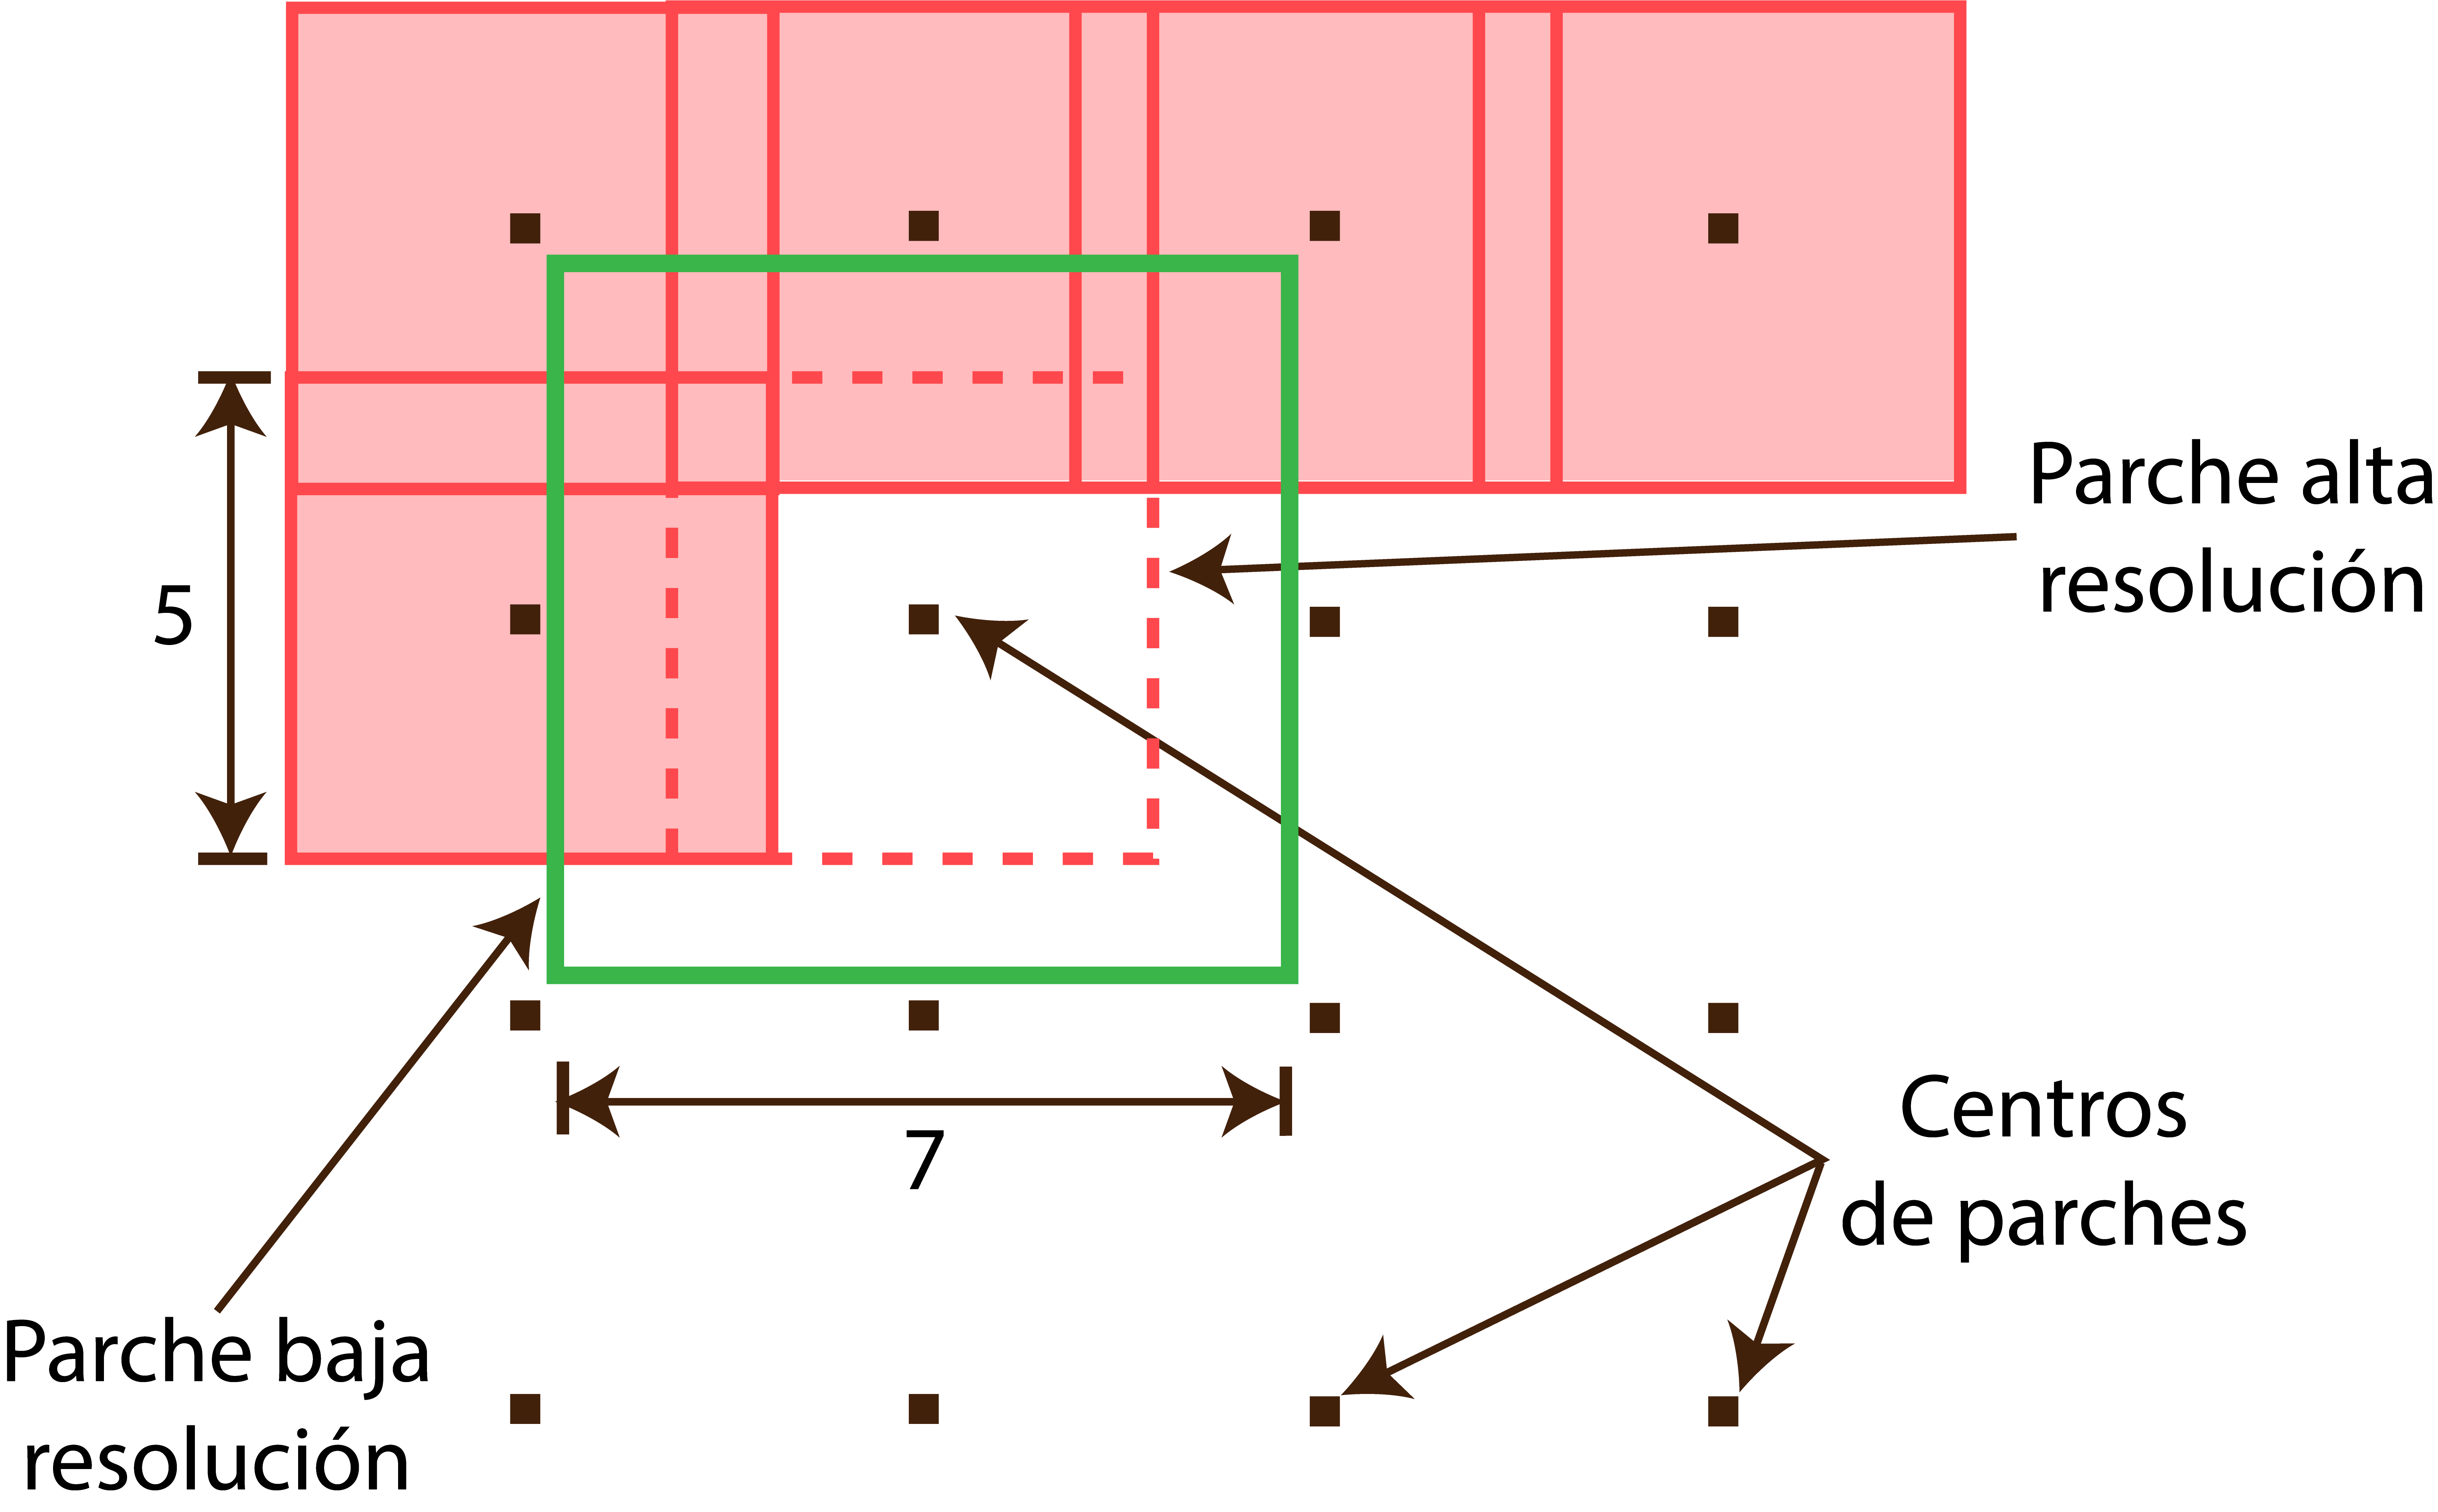
\includegraphics[scale = 0.3]{ fr_diccionario.png }
    \centering
    \caption{ Adquisición de parches de cada imagenes}
    \label{fig:fr_dic}
\end{figure}

En específico, los parches de baja resolución deben reordenarse como un vector 
en $\mathbb{R}^{1\times49}$ concatenado con la primera fila y primera columna
del parche de alta resolución, resultando en un vector en $\mathbb{R}^{1\times59}$.
Lo último es necesario para considerar la superposición
de los parches de alta resolución de la imagen a reconstruir. 

Cabe destacar que la base de entrenamiento está en 
RGB por lo que bastará con el procedimiento antes mencionado para guardar
los pares de parches en algún archivo de fácil acceso. 

\subsubsection{Algoritmo de predicción}
\noindent
Una vez teniendo el diccionario o base de entrenamiento es necesario establecer el algoritmo de 
predicción para generar esos detalles no visibles en la imagen original.
Para ello, la imagen de entrada (en baja resolución) debe ser pre-procesada
mediante un filtro pasa-altas para eliminar información innecesaria y posteriormente realizar
un proceso de escalado mediante algún algoritmo de interpolación para
aumentar sus dimensiones y densidad de los pixeles tal como se presenta
en la Figura \ref{fig:fr_algoritmo}. Observe que para ese punto, la imagen de entrada
cuenta con los píxeles que representan sus bordes o detalles que han sido
escalados con el objetivo de tener una base a partir de la cual se va a reconstruir
con más detalle la imagen de salida.  

Puesto que \cite{freeman} propone que la reconstrucción sea con parches, se debe 
realizar una búsqueda para elegir al parche de la base de datos que se aproxime 
más al parche de entrada con el objetivo de realizar la reconstrucción. En la
Figura \ref{fig:fr_prediccion} se observa el algoritmo propuesto por
\emph{Freeman et al} para la predicción de parches.

\begin{figure}[H]
    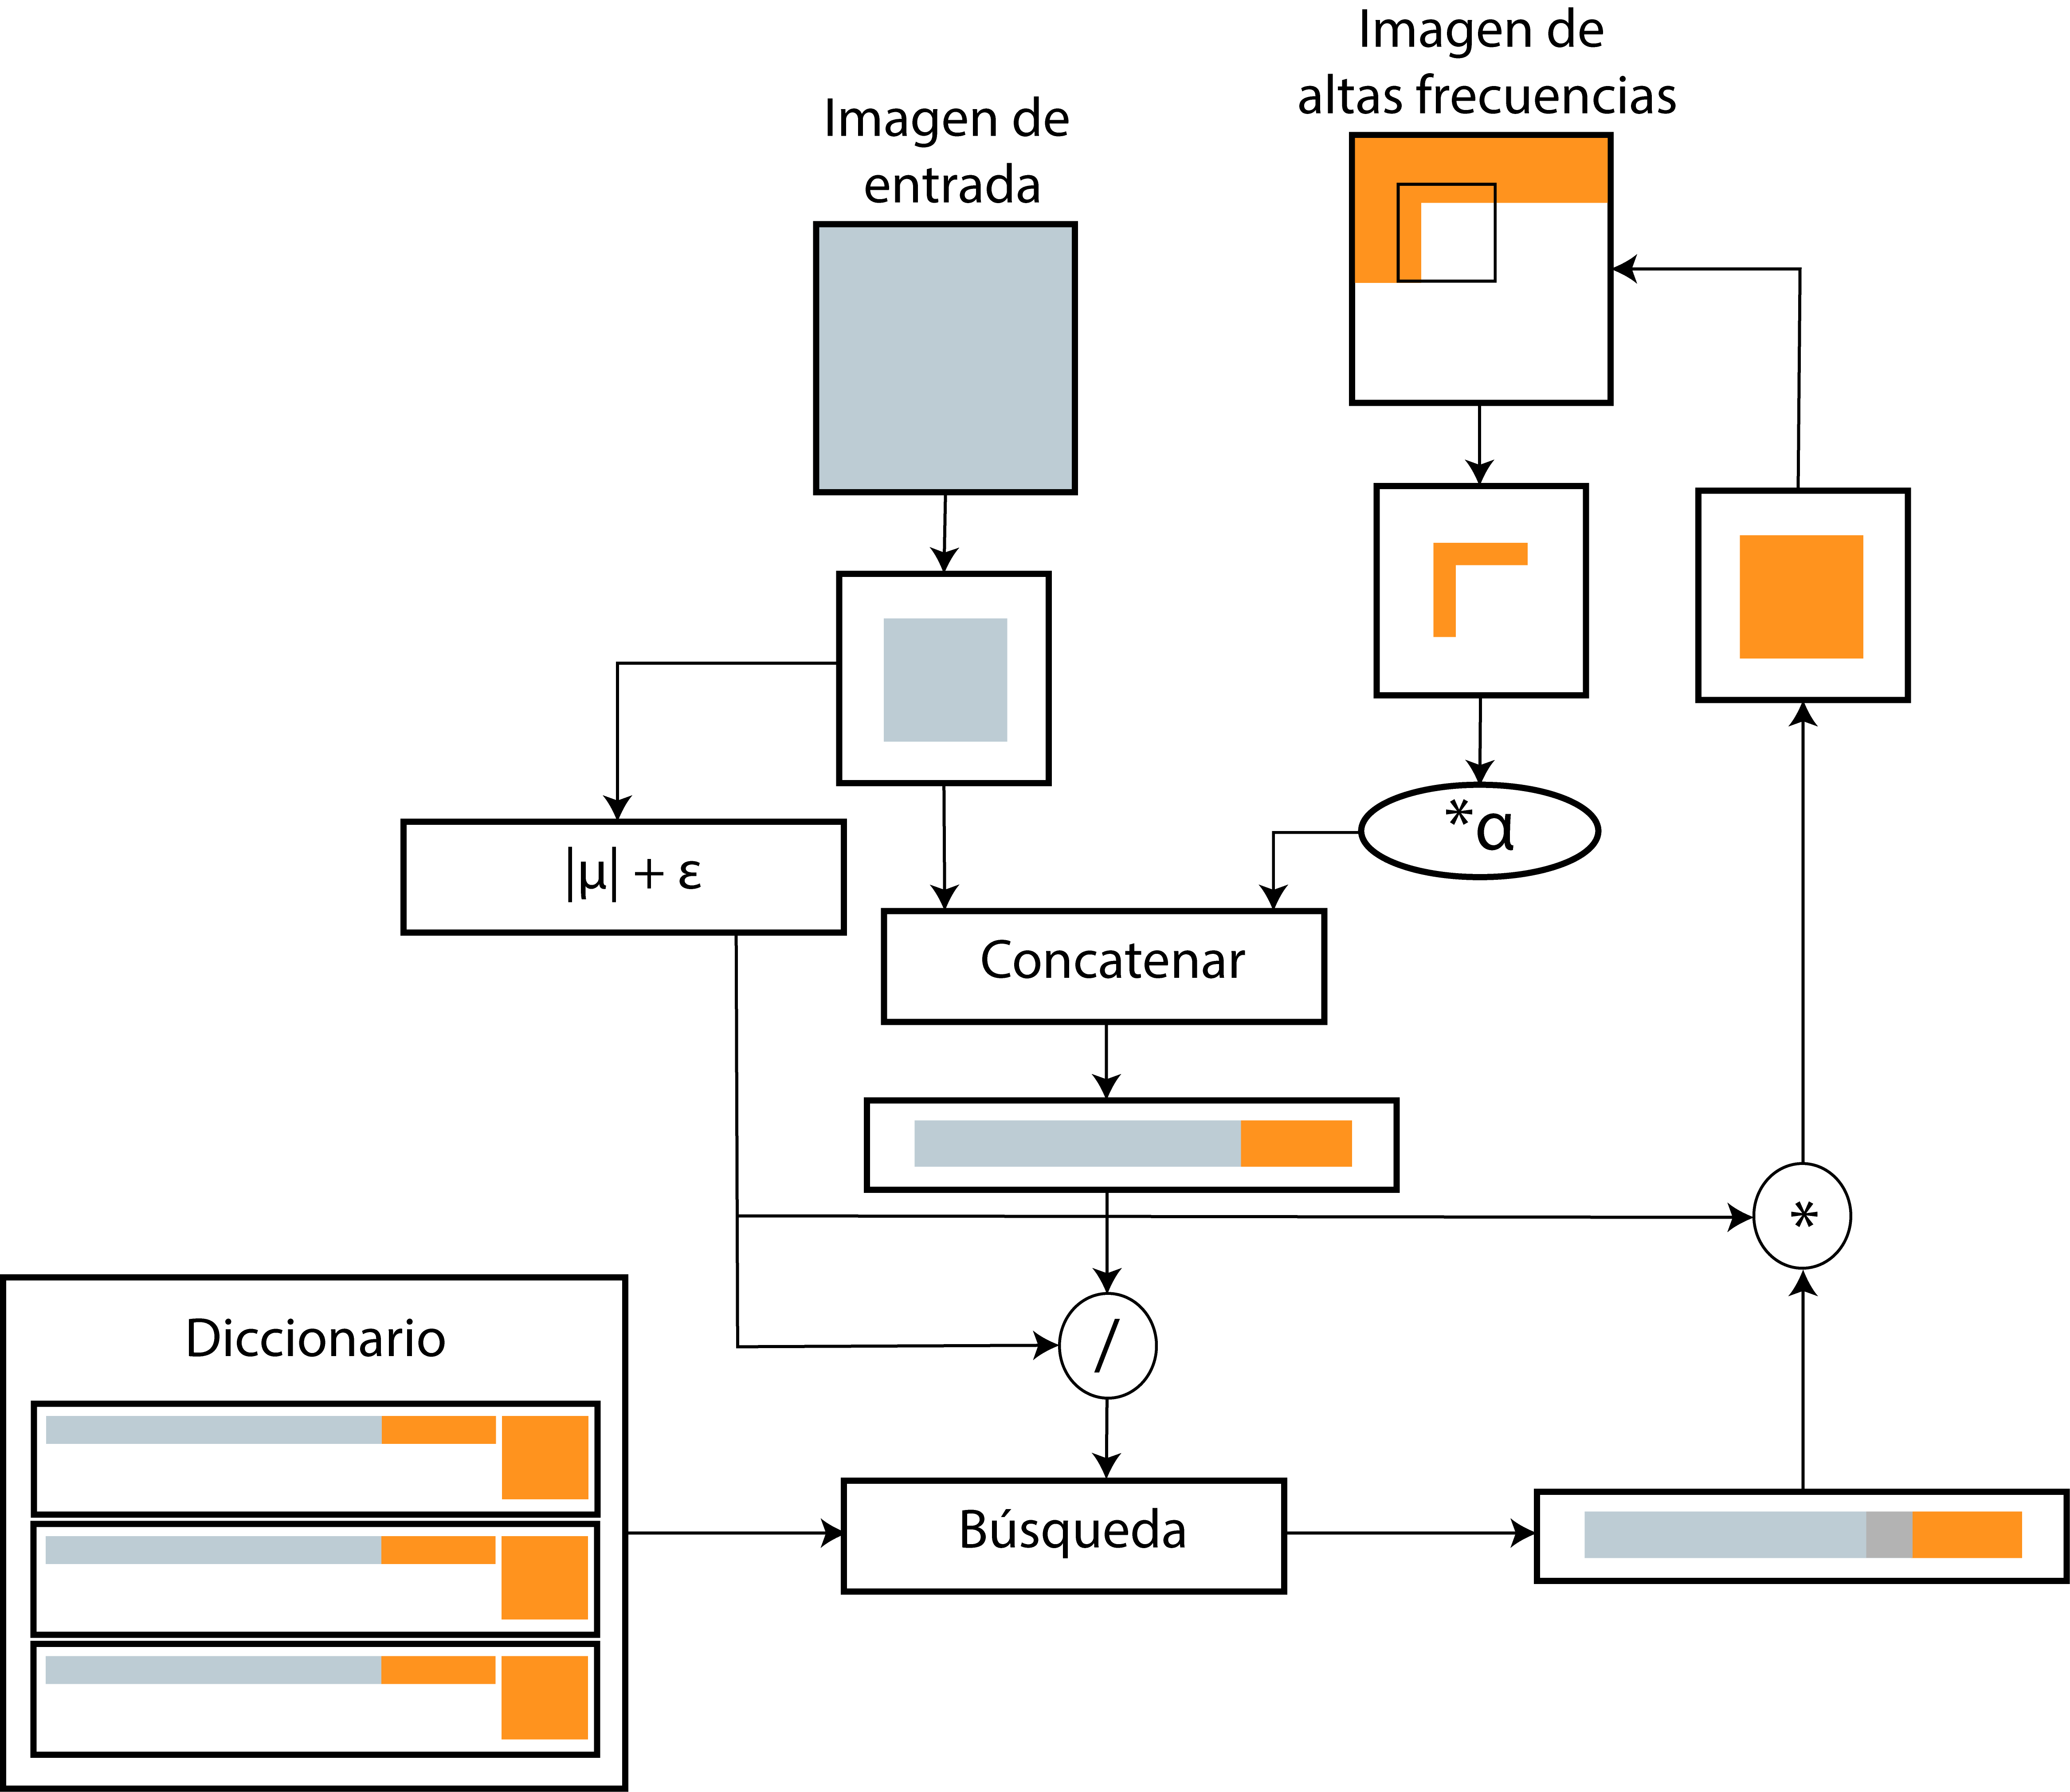
\includegraphics[scale = 0.5]{ freeman_prediccion.png}
    \centering
    \caption{ Algoritmo de predicción de imagen de frecuencias altas }
    \label{fig:fr_prediccion}
\end{figure}

Observe que la imagen de entrada se irá segmentando en los parches de baja 
resolución (color gris-verdoso). Estos parches se calculará su media absoluta 
$|\mu|$ más un $\epsilon$ (para evitar indeterminación ante parches con poco
contraste), posteriormente se concatena con el producto del factor de control 
$\alpha$ que considera la \emph{superposición} entre los parches de alta resolución
(naranjas). Dicha concatenación se divide entre el promedio absoluto más $\epsilon$
para convertirse en el vector a buscar en el diccionario. 

Dada la gran combinación de valores, resulta bastante complicado encontrar 
exactamente el mismo vector en el diccionario previamente construido y por
lo mismo se utilizan algoritmos de búsqueda aproximados como el del \emph{vecino
más cercano}. Esto puede observarse en la salida del algoritmo al notar que el 
vector emparejado tiene un pixel de color diferente al solicitado, pero como 
es muy cercano, resulta la salida del algoritmo de búsqueda. 

Dicho vector de búsqueda permite emparejar al parche de alta resolución asociado
en el diccionario, el cual será multiplicado por el factor $|\mu|+\epsilon$ para 
retomar las tonalidades del parche de baja resolución e incrustado en la \emph{imagen de altas frecuencias}
para ejecutar nuevamente el algoritmo de manera iterativa.

De acuerdo con \cite{freeman}, el \emph{algoritmo de un paso} evita considerar
los parches como variables aleatorias y relacionarlas con \emph{Redes de Markov}
considerando el algoritmo \emph{belief propagation}. Esto es una enorme ventaja,
ya que se simplifica el proceso de selección del parche considerando 
únicamente la \emph{superposición} futura en los parches de alta resolución. 

\subsubsection{Imagen de alta resolución}
\noindent
Finalmente, como resultado del algoritmo propuesto en \cite{freeman} se obtiene
una imagen de mejor resolución que la entrada considerando un factor de escalado
deseado para el proceso de interpolación. Note que el motor central del algoritmo
está basado en el algoritmo de predicción descrito anteriormente y el diccionario
construido a partir de un conjunto de imágenes donde se realizará la búsqueda
mediante el algoritmo del \emph{vecino más cercano}. 

Como producto del algoritmo de predicción se obtendrá una imagen con sólo frecuencias
altas que no se encontraban explícitamente en la imagen de entrada y que se sumará
con la imagen escalada para obtener así la imagen de alta resolución respecto
la imagen de entrada tal como se observa en la Figura \ref{fig:fr_algoritmo}.
    % Descripción de lo que es una red convolucional
\subsection{Redes neuronales}
Las redes neuronales \cite{RedesNeuronales}, también conocidas como redes neuronales artificiales (ANN) o redes neuronales simuladas (SNN),
son un subconjunto de machine learning y están en el corazón de los algoritmos del deep learning. Su nombre y estructura están
inspirados por el cerebro humano, imitando la forma en que las neuronas biológicas se señalan entre sí.\\
Las redes neuronales artificiales (ANN) están compuestas por capas de nodos, que contienen una capa de entrada, una o más
capas ocultas, y una capa de salida. Cada nodo, o neurona artificial, se conecta a otro y tiene un peso y un umbral asociados.
Si la salida de cualquier nodo individual está por encima del valor de umbral especificado, dicho nodo se activa, enviando datos
a la siguiente capa de la red. De lo contrario, no se pasan datos a la siguiente capa de la red. En la figura \ref{fig:SRCNN_RedNeuronal}
se muestra la estructura general de una red neuronal.

\begin{figure}[H]
    \centering
    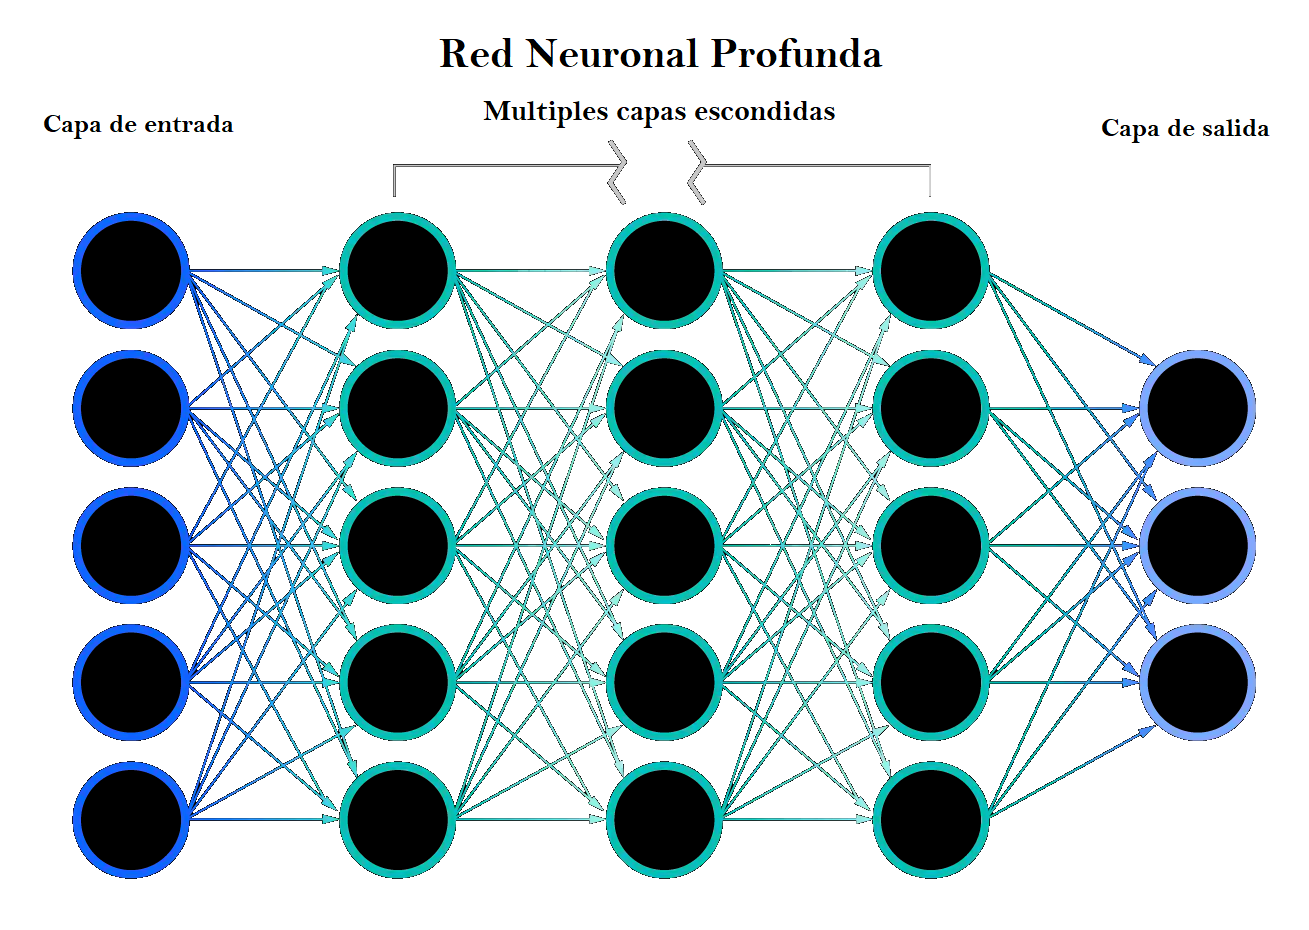
\includegraphics[scale=0.5]{Red_Neuronal.png}
    \caption{Estructura de una red neuronal}
    \label{fig:SRCNN_RedNeuronal}
\end{figure}

Cada nodo o neurona de la red recibe datos de entrada $x_i$ y realiza la suma mediante ponderaciones $w_i$, además de agregar un
sesgo $bias$ y finalmente nos da una salida $f(x)$ solo si $f(x)\geq umbral$, de lo contrario la salida será $0$.

\begin{align}
    \label{eqn:SRCNN_RedNeuronal}
                 x&=\sum_{i=1}^{m}\omega_ix_i+bias
\end{align}
%\begin{align}
%    \nonumber    f(x)&=\left\lbrace\begin{equation}
%                       f(x)\hspace{0.5cm}si\hspace{0.1cm}f(x)>=umbral \\
%                       0\hspace{1.0cm}si\hspace{0.1cm}f(x)<umbral \\
%                    \end{equation}\right.
%\end{align}

\subsection{Redes Convolucionales}
\noindent
Las Redes neuronales convolucionales \cite{RedesConvolucionales} son  un tipo de redes neuronales artificiales  donde las \emph{neuronas}
corresponden a campos receptivos de una manera muy similar a las neuronas en la corteza visual primaria de un cerebro
biológico.  Este tipo de red es una variación de un perceptrón multicapa, sin embargo, debido a que su aplicación es realizada
en matrices bidimensionales, son muy efectivas para tareas de visión artificial, como en la clasificación y segmentación 
de imágenes, entre otras aplicaciones.
Las redes neuronales convolucionales consisten en múltiples capas de filtros convolucionales de una o más dimensiones. Después de
cada capa, por lo general se añade una función para realizar un mapeo causal no-lineal.\\
Como cualquier  red empleada para clasificación, al principio estas redes tienen una  fase de extracción de características,
compuesta de neuronas convolucionales , luego hay una reducción por muestreo y al final tendremos neuronas de perceptrón mas
sencillas para realizar la clasificación final sobre las características extraídas.\\
La fase de extracción de características se asemeja al proceso estimulante en las células de la corteza visual. Esta fase se
compone de capas alternas de neuronas convolucionales y neuronas de reducción de muestreo. Según progresan los datos a lo largo
de esta fase, se disminuye su dimensionalidad, siendo las neuronas en capas lejanas mucho menos sensibles a perturbaciones en
los datos de entrada, pero al mismo tiempo siendo estas activadas por características cada vez más complejas.\\

\subsubsection{Convolucion}
Ahora comienza el \emph{procesado distintivo} de las Redes neuronales convolucionales, es decir, haremos las llamadas
\emph{convoluciones}: Estas consisten en tomar \emph{grupos de pixeles cercanos} de la imagen de entrada e ir operando
matemáticamente (producto escalar) contra una pequeña matriz que se llama kernel.  Ese kernel supongamos que tiene un tamaño
de $3\times 3$ pixels y con ese tamaño logra \emph{visualizar} todas las neuronas de entrada (de izquierda-derecha, de arriba-abajo)
y asi logra generar una nueva matriz de salida, que en definitiva será nuestra nueva capa de neuronas ocultas.\\

\begin{figure}[H]
    \label{fig:SRCNN_Convolucion}
    \centering
    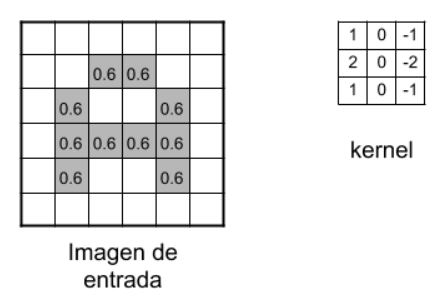
\includegraphics{Convolucion.png}
    \caption{Convolución con \textbf{kernel} de $3\times 3$}
\end{figure}

\subsubsection{Decenso del gradiente}
Para que la red neuronal convolucional \emph{aprenda} se hace uso del algoritmo \emph{backpropagation}, el cual emplea el
algoritmo del descenso del gradiente \cite{DescensoGradiente}, el cual es de uso general y se encarga, de forma numérica, de encontrar un mínimo de
de funciones multivariadas.\\

\begin{figure}[H]
    \label{fig:SRCNN_GradDescent}
    \centering
    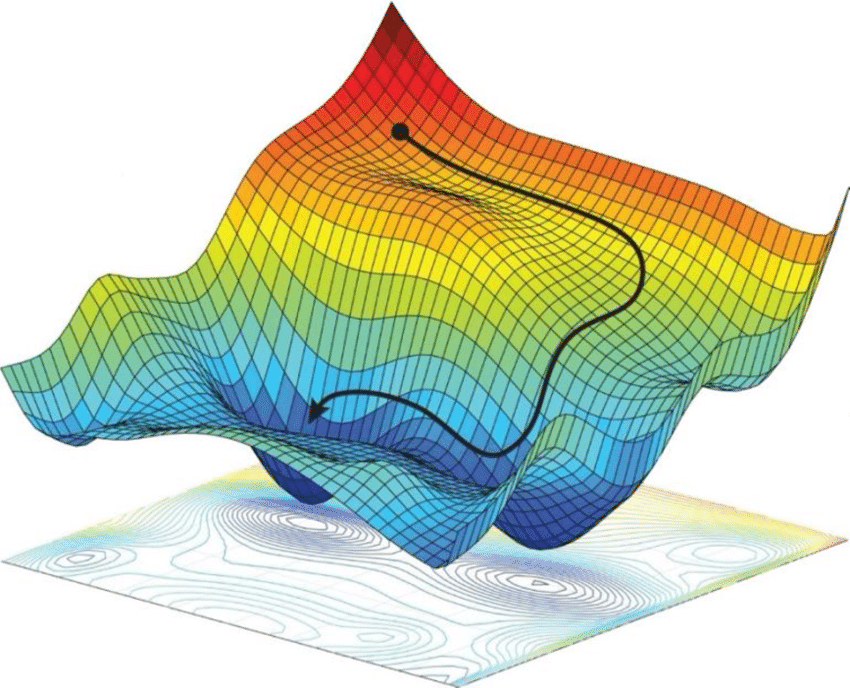
\includegraphics[scale=0.2]{Grad_Des_1.png}
    \caption{Descenso del gradiente}
\end{figure}

Para minimizar la función, podemos seguir el negativo del gradiente, y así ir en la dirección del descenso más pronunciado.
Este es el descenso del gradiente. Formalmente, si comenzamos en un punto $x_0$ y nos movemos una distancia positiva $\alpha$
en la dirección del gradiente negativo, entonces nuestro nuevo y \emph{mejorado} $x_1$ se verá como $x_1=x_0-\alpha\nabla f(x_0)$.
De manera general, podemos definir esto como:

\begin{align}
    \label{eqn:SRCNN_DescensoGradiente}
    x_{n+1}=x_n-\alpha\nabla f(x_n)
\end{align}

\subsubsection{Optimizador Adam (Estimación Adaptiva de Momentos)}
Lo que un optimizador \cite{AdamOptimizador} hace es mejorar los valores de los parámetros de la red con el fin de reducir el error cometido por la red.
Para ello se utiliza (Como se mencionó en el descenso del gradiente) el algoritmo de \emph{backpropagation}.\\
El optimizador más básico posible es actualizar los valores de los parámetros, equitativamente, con base en la \textbf{tasa de
aprendizaje} (\emph{learning rate}), el cual es presentado en \eqref{eqn:SRCNN_DescensoGradiente}, en donde la tasa de aprendizaje
corresponde al parámetro \textbf{$\alpha$} y es un valor constante.\\
El optimizador \textbf{Adam} es un adaptador que pertenece a la familia de \textbf{optimizadores adaptativos}, surge de la
combinación de otros 2 adaptadores pertenecientes a esta familia: \textbf{RMSProp} y \textbf{Momentum}.
El adaptador adam quedá descrito por la siguiente ecuación:

\begin{equation}
    \label{eqn:SRCNN_Adam}
    \begin{split}
        m&=\beta_1m+(1-\beta_1)\nabla W\\
        v&=\beta_2v+(1-\beta_2)\nabla W^2\\
        W&=W-\frac{\alpha m}{\sqrt{v+\epsilon}}
    \end{split}
\end{equation}

Donde en la ecuación \eqref{eqn:SRCNN_Adam} $m$ y $v$ representan los dos momentos, siendo $m$ el que modela la media de los
gradientes a lo largo del tiempo, mientras que $v$ hace lo mismo con la varianza. Por lo general los valores de $\beta_1$ y
$\beta_2$ se fijan como: $\beta_1=0.9$, $\beta_2=0.999$. El parámetro $\alpha$ corresponde a la tasa de aprendizaje, $W$
representa los parámetros de la red y finalmente el parámetro $\epsilon$ es un valor pequeño utilizado para evitar el
truncamiento numérico.

\subsubsection{Error Cuadrático Medio (MSE)}
Mientras entrenamos el modelo, vamos a querer evaluar su precisión usando una función de costo (o pérdida). Esto también
se conoce comúnmente como el error cuadrático medio (MSE). Este se obtiene de la siguiente expresión:

\begin{align}
    \label{eqn:SRCNN_MSE}
    MSE=\frac{1}{2m}\sum_{i=1}^{m}(\hat{y}_i-y_i)^2
\end{align}

Donde en la ecuación \eqref{eqn:SRCNN_MSE}; $i$ representa el indice de la muestra, $\hat{y}$ es el resultado previsto,
$y$ es el valor real y  $m$ es el número de muestras.\\
En última instancia, el objetivo es minimizar nuestra función de costo para asegurar la correción de ajuste para cualquier
observación dada. A medida que el módelo ajusta sus ponderaciones y sesgos, utiliza la función de costo  y el aprendizaje
de refuerzo para alcanzar el punto de convergencia, o el mínimo local. El proceso en el que el algoritmo ajusta sus
ponderaciones es a través del descenso del gradiente (o el optimizador \textbf{Adam}), lo que permite que el módelo
determine la dirección a tomar para reducir los errores (o minimizar la función de costo). Con cada ejemplo de entrenamiento,
los parámetros del módelo se ajustan para converger gradualmente al mínimo.

\begin{figure}[H]
    \label{fig:SRCNN_MSE}
    \centering
    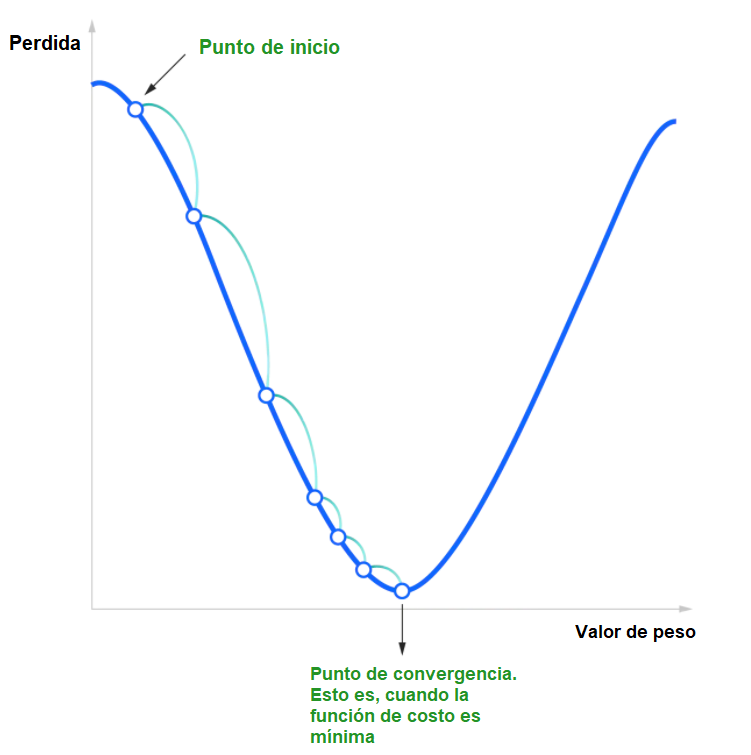
\includegraphics[width=10cm, height=6cm]{MSE.png}
    \caption{Minimización de función de costo (MSE)}
\end{figure}
    \subsection{SRGAN}

El SISR (Single Image Super Resolution) es un problema inverso, \emph{it est}, que para una imagen de baja resolución puede haber muchas
imágenes diferentes de alta resolución que le correspondan, esto basado en la interpretación del método utilizado, ya que
el principio básico es añadir información para obtener imágenes de alta resolución.
Las CNN presentan un gran avance en la reconstrucción de imágenes de baja resolución a alta resolución,
sin embargo, debido al escalado de la imagen o el hecho de que la imagen que se busca mejorar presenta grandes
variaciones con respecto a las del dataset (\emph{Data Augmentation}) los resultados podrían ser no satisfactorios.


Una alternativa que propone un nuevo paradigma son las GAN´s (Generative Adversarial Networks), cuyo funcionamiento está basado
en la estimación de modelos generadores, como mencionan Goodfellow et al. \cite{GANs}, esto es 
posible gracias al entrenamiento simultáneo de dos modelos, uno \emph{generador (G)} que obtiene 
la distribución de la entrada para generar datos falsos y el otro \emph{discriminador (D)} el cual se encarga de estimar 
la probabilidad de que la muestra provenga del dataset de entrenamiento y discernir así entre estos datos y 
los del modelo \emph{ generador (G)}.

El término \emph{antagónicas} como se menciona en \cite{SRGAN_Tesis}, se refiere a la dinámica 
competitiva que se mantiene entre los dos modelos. Por un lado,
el generador tiene por objetivo crear nuevos datos que sean indistinguibles del
conjunto de entrenamiento, mientras que el discriminador debe poder ser capaz
de distinguir cuáles son los datos creados y los reales, siendo los últimos los que corresponden
 al conjunto de entrenamiento. Esto resulta en un proceso iterativo donde estos dos modelos
 se desafían uno a otro, logrando un ajuste de parámetros
 que logran producir datos que se parezcan con gran acierto a los reales.
 

\begin{figure}[H]
    \begin{center}
      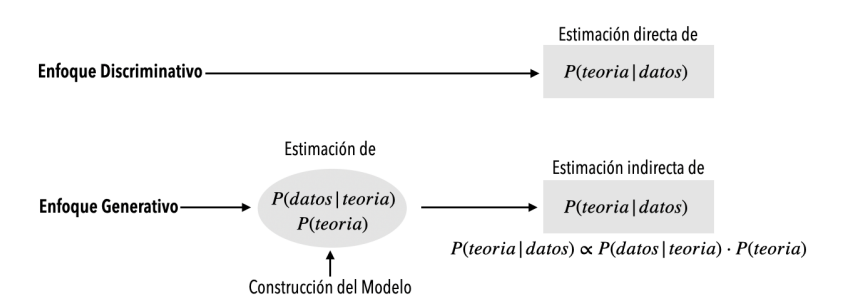
\includegraphics[scale = 0.9]{modelo_gen_disc.png}
      \caption{Modelo Generador y Discriminador}
      \label{Alexis1}
    \end{center}
\end{figure}


El modelo SRGAN (Super Resolution Generative Adversarial Network) fue
propuesto en 2016 por un grupo de investigadores\cite{SRGAN}.
La principal innovación de este modelo es su función de pérdida, llamada
función de pérdida perceptual, que permite mejorar el realismo de la imagen de
salida.

\subsubsection{Componentes.}

Profundizando un poco más en los componentes del algoritmo, en especifico, el uso de las \emph{GAN´s} para la obtención de Super-Resolución (\emph{SRGAN}), 
tenemos al discriminador el cual es una red neuronal convolucional que consta de muchas 
capas ocultas y una capa de salida, la principal diferencia aquí es que la capa de salida de las GAN puede tener solo dos salidas, 
a diferencia de las CNN, que pueden tener un número diferente de salidas con respecto a la cantidad de etiquetas en las que está entrenado.
La salida del discriminador puede ser 1 o 0 dependiendo de la función de activación que se aplique. Si la salida es 1, 
entonces los datos proporcionados son reales y si la salida es 0, entonces se refiere a ellos como datos falsos.

El discriminador está capacitado con los datos del dataset, con estos aprende a reconocer cómo se ven y qué características deben 
clasificarse como reales, formalmente, discrimina entre $\tilde{x}$, la muestra falsa, y $x$, 
los datos muestreados de la distribución real de datos $P_{datos}(x)$.




\begin{figure}[H]
    \begin{center}
      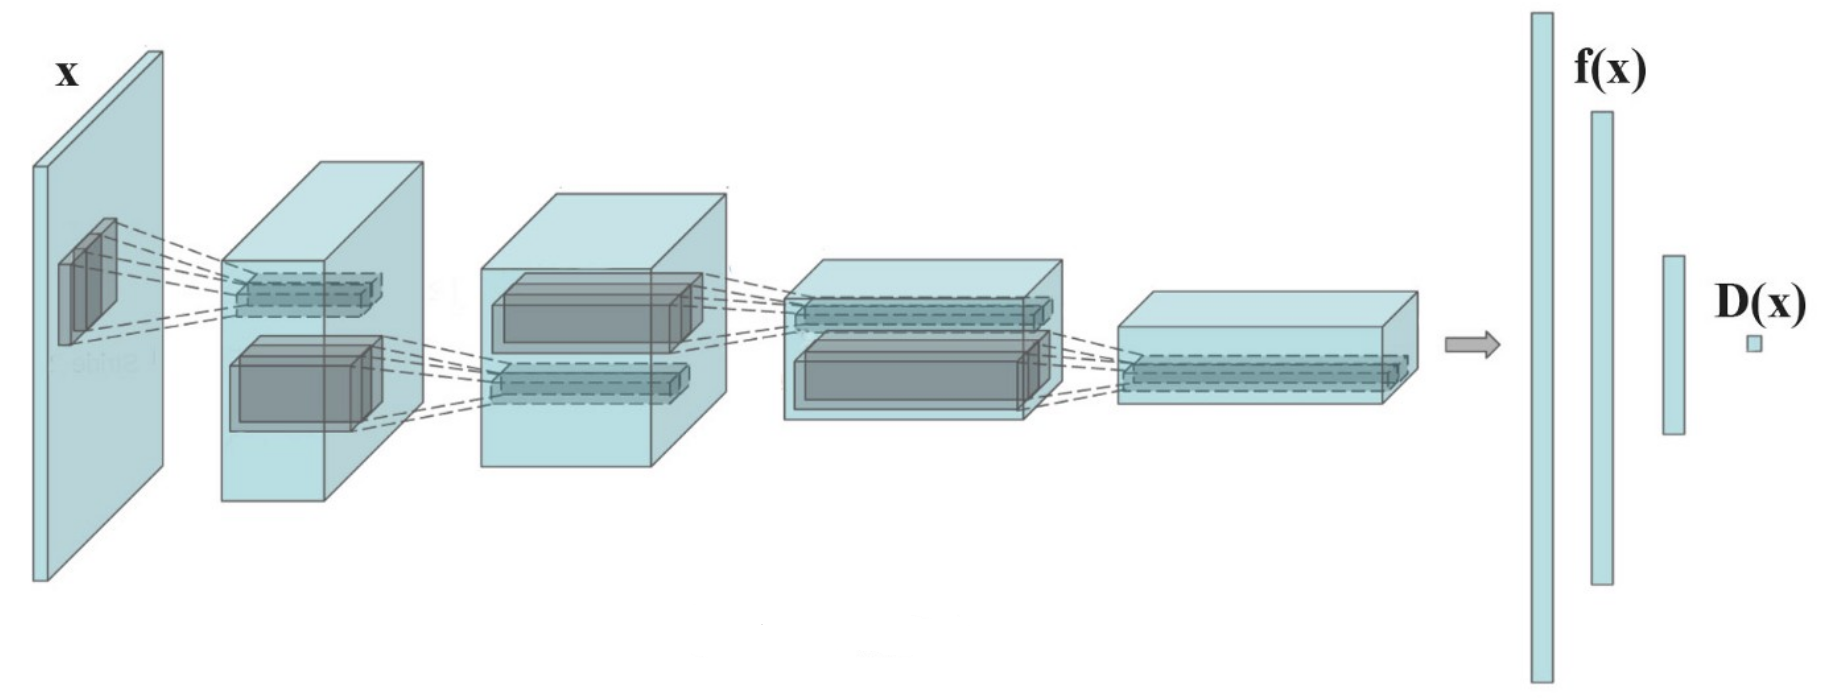
\includegraphics[scale = 0.4]{discriminador.png}
      \caption{Modelo Discriminador}
      \label{Alexis2}
    \end{center}
\end{figure}


Por el contrario, el generador es una red neuronal convolucional inversa, hace exactamente lo opuesto de lo que hace una CNN, ya que 
a estas se les da una imagen real como entrada y se espera una etiqueta clasificada como salida, 
pero en el generador, un vector de ruido aleatorio\emph{(z)} se da como señal de entrada 
y se espera una imagen falsa como salida, esta imagen deberá aproximarse a la real a
partir de una distribución $P(z)$ (en general una distribución Gaussiana) que
produce una muestra de datos falsos,$\tilde{x}$ es decir:

\begin{equation}
G(z) = \tilde{x}
\end{equation}

\begin{figure}[H]
    \begin{center}
      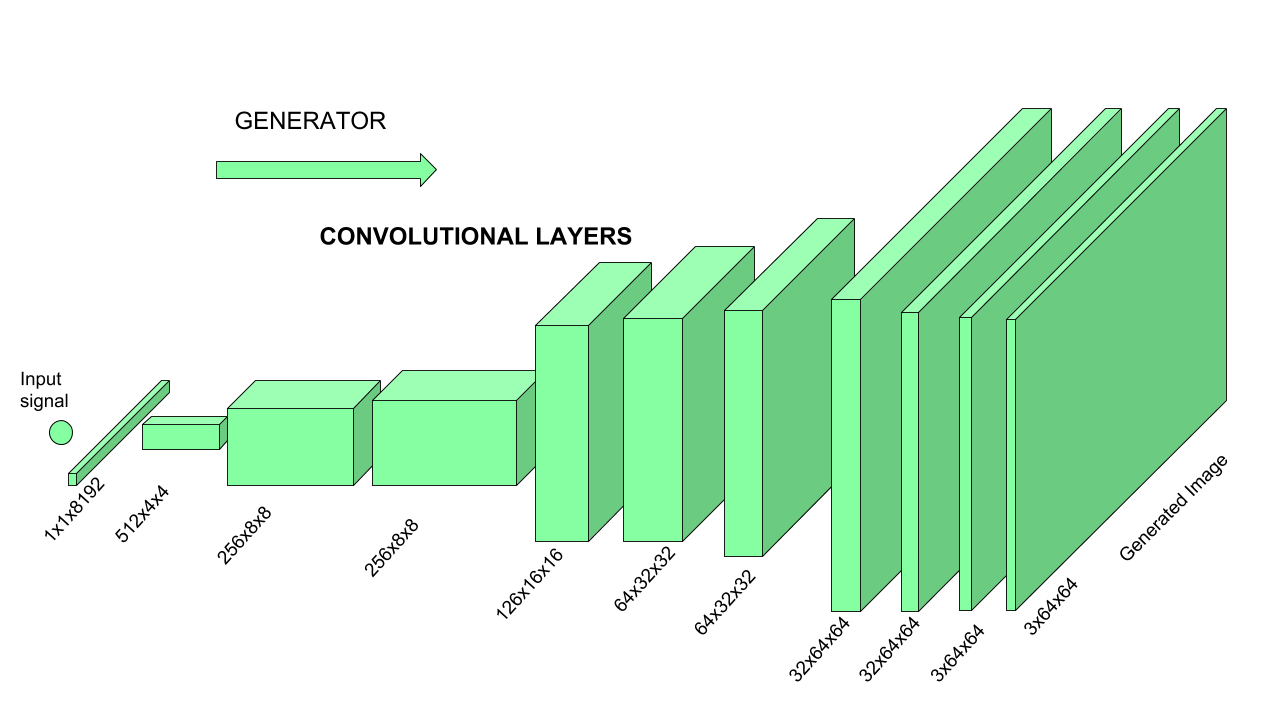
\includegraphics[scale = 0.6]{generador.png}
      \caption{Modelo Generador}
      \label{Alexis3}
    \end{center}
\end{figure}
    
\subsubsection{Funciones de perdida.}

Como parte del entrenamiento se necesitan parámetros que nos describan de manera correcta los resultados
que obtenemos de la predicción en nuestra red neuronal, para esto se hace el uso de funciones de perdida, estas funciones 
evalúan la desviación entre las predicciones realizadas por la red neuronal y los valores 
reales de las observaciones utilizadas durante el aprendizaje. A esta función se le conoce como perdida perceptual. Cuanto menor es el resultado de esta función, 
más eficiente es la red neuronal. Su minimización, es decir, reducir al mínimo la desviación entre el valor de la predicción y
el valor real para una observación dada, se hace ajustando los distintos pesos de la red neuronal.

En el caso de las redes adversarias, específicamente en \emph{SRGAN}, esta perdida es la suma de las perdidas de contenido $l_{X}^{SR}$ 
y las adversarias $10^{-3}l_{Gen}^{SR}$.


\begin{equation}
  l^{SR}=l_{X}^{SR} + 10^{-3}l_{Gen}^{SR}
\end{equation}


Como mencionan Goodfellow et al. \cite{GANs}, se tienen 
2 perdidas principales: La de contenido (\emph{content loss}), la cual se aproxima a una perdida perceptual mediante la perdida
de la red neuronal (\emph{VGG}),definimos entonces la perdida \emph{VGG} como la distancia euclidiana entre la representación de
características de una imagen reconstruida $G_{\theta G}(l^{LR})$ y la imagen de referencia o real $l^{HR}$.


\begin{equation}
  l_{VGG/i.j}^{SR}=\frac{1}{W_{i,j}H_{i,j}} \sum_{x=1}^{W_{i,j}}\sum_{y=1}^{H_{i,j}}(\phi_{i,j}(l^{HR})_{x,y}-\phi_{i,j} 
  (G_{\theta G}(l^{LR}))_{x,y})^{2}
\end{equation}

Por otra parte tenemos la perdida adversaria, esta se añade el componente generador de nuestro modelo GAN a la perdida perceptual,
esto promueve que nuestra red cree soluciones que engañen al discriminador. Las perdidas del generador $l_{Gen}^{SR}$ se definen
en base a las probabilidades del modelo discriminador $D_{\theta D}(G_{\theta G}(l^{LR}))$ sobre las muestras de entrenamiento
de la siguiente manera:

\begin{equation}
  l_{Gen}^{SR}=\sum_{n=1}^{N}-log \ D_{\theta D}(G_{\theta G}(l^{LR}))
\end{equation}


Donde $D_{\theta D}(G_{\theta G}(l^{LR}))$ es la probabilidad de que nuestra imagen reconstruida $G_{\theta G}(l^{LR})$ sea 
una imagen de alta resolución y la función logarítmica nos ayuda con el comportamiento del gradiente. 


    % Descripción de la SRCNN
\subsection{Red Neuronal Convolucional de Super Resolución: (SRCNN por sus siglas en inglés)}
Como se menciona en \cite{freeman}, tradicionalmente se utilizan 3 etapas para la super resolución de imagenes:
\begin{enumerate}
    \item Extracción de parches en baja resolución y representación en un vector de "alta" dimensión
    \item Mapeo entre vectores (parches de baja resolución) de baja resolución con vectores que representan parches de alta
    resolución
    \item Reconstrucción de imagén
\end{enumerate}
Estas 3 etapas generalmente se realizan por separado, es por ello que se propone el uso de una red convolucional en la cual se
lleven a cabo estas 3 operaciones de manera conjunta.\\
En \cite{SRCNN} se propone una red convolucional que consté de 3 capas, cada una correspondiente a las etapas que clasicamente
se siguen para el problema de super resolución, es decir, 1) Se diseña una primer capa convolucional con la cual se busca la
"extracción" de los parches de baja resolución, 2) una capa que estará conectada directamente con la salida de la primer capa
convolucional, y que será la encargada de realizar el "mapeo" entre los parches de baja resolución y los parches de alta
resolución y 3) una capa final encargada de realizar la reconstrucción de la imagen de alta resolución.

\begin{figure}[H]
    \label{fig:SRCNN_Arquitectura}
    \centering
    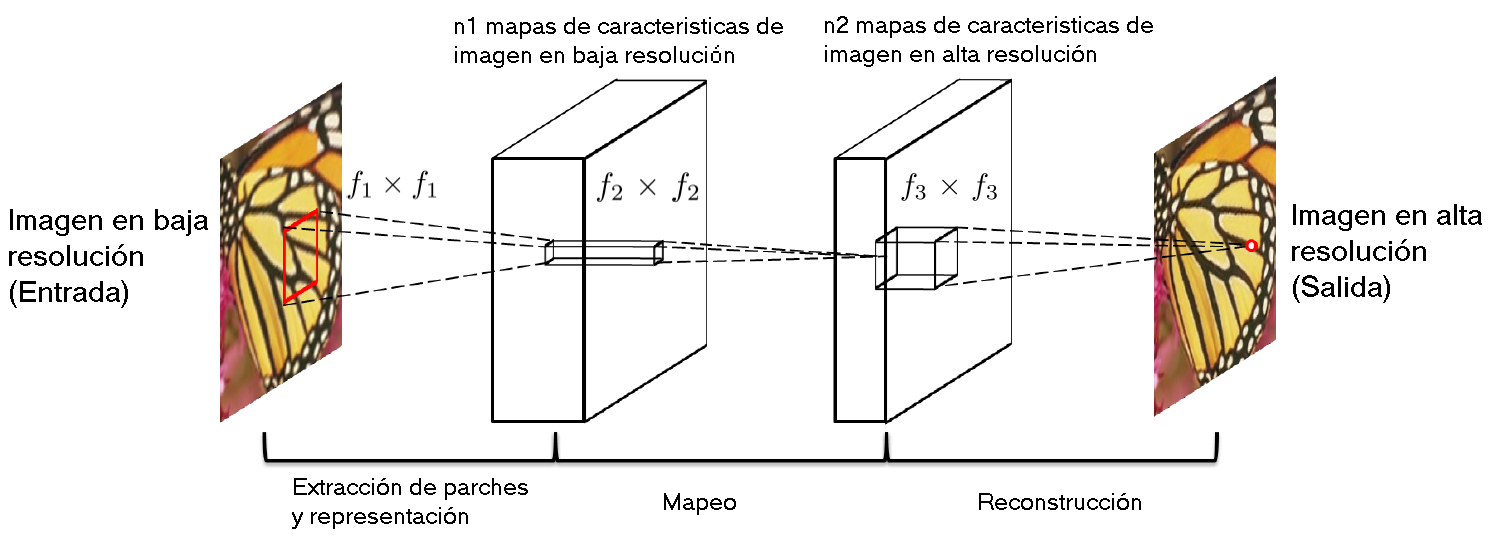
\includegraphics[scale = 0.6]{SRCNN_Arquitectura.png}
    \caption{Arquitectura de la SRCNN}
\end{figure}

Se busca generar un mapeo entre directo entre la imagen de baja resolución (Y) y la de alta resolución real (X).

\textbf{1. Extracción de parches}\\
Esta etapa comunmente se basa en la extracción de parches de baja resolución y representarlos por un conjunto de bases pre-entrenadas
tales como PCA,DCT,Haar,etc. Esto es equivalente a "convolucionar" la imagen por un conjunto de filtros, donde cada uno de estos
representaria las bases pre-entrenadas. En la formulación de la SRCNN, se envuelve la optimización de estas bases en la optimización
de la red. Formalmente, la primer capa se expresa como una operación $F_1$:
\begin{align}
    \label{eqn:SRCNN_FirstLayer}
    F_1(Y)=max(0,W_1*Y+B_1)
\end{align}
Donde $Y$ y $B_1$ representan los filtros y el \emph{bias} respectivamente y el operador "$*$" denota la operación de convolución.
Se utiliza la función de activación \textbf{ReLU} (ReLU,$max(0,x)$) en las respuestas de los filtros.\\

\textbf{Mapeo}\\
La primer capa extrae caracteristicas de $n_1$ dimensiones para cada parche. En la segunda operación se realiza un mapeo de cada
uno de estos vectores de dimensiones $n_1$ con vectores de dimensiones $n_2$. Esto es equivalente a aplicar $n_2$ filtros. Esta
descripción es válida para filtros de kernel $1\times1$, pero es facil generalizar para otros tamaños de \emph{kernel}, solo que
ahora el mapeo se realiza en parches de kernel $p\times p$. La operación de la segunda capa es:

\begin{align}
    \label{eqn:SRCNN_SecondLayer}
    F_2(Y)=max(0,W_2*F_1(Y)+B_2)
\end{align}

Cada uno de los vectores de salida de dimensiones $n_2$ es conceptualmente la reprsentación de un parche en alta resolución que
será utilizado para la reconstrucción.\\

\textbf{Reconstrucción}\\
En los métodos tradicionales, la predicción de traslapamiento de parches de alta resolución es frecuentemente promediada para
producir la imagen final. El promediado puede ser considerado como un filtro pre-definido sobre un conjunto de mapas de
características (Donde cada posición es la forma de vector "aplando" de un parche de alta resolución). Se define una capa
convolucional para producir la imagen final en alta resolución:

\begin{align}
    \label{eqn:SRCNN_ThirdLayer}
    F(Y)=W_3*F_2(Y)+B_3
\end{align}


    \section{Implementación}
    \noindent
Dado que el objetivo del proyecto es comparar tres diferentes métodos 
de súper resolución, en esta sección se presentarán las actividades
requeridas para la implementación de los métodos. Considerando desde los 
requisitos de software, hardware y datos de entrenamiento en caso sean 
necesarios. 

\subsection{Example-Based Super-Resolution}
\noindent
Para el primero de ellos, se retoma la literatura expuesta en \cite{freeman}
comenzando con la generación del diccionario donde se encuentran relacionados 
los parches de baja y alta resolución. Previo a esto, es necesario pre-procesar
el conjunto de imágenes para su posterior segmentación. 

De acuerdo a las indicaciones, se deben tener pares de imágenes en alta y baja 
resolución. En particular, se ha considerado las primeras 13 imágenes del 
\emph{dataset} disponible en \cite{MIRFLICKR}.

Realizando un método iterativo que realiza un barrido bidimensional en cada imagen
resulta bastante sencillo obtener los parches correspondientes de alta y baja resolución. 

    \subsection{SRCNN}
Partimo del método descrito en \cite{SRCNN}, en el cual se menciona una red que cuente con al menos 3 capas convolucionales, de
manera que la primer capa se encargue de extraer los parches de baja resolución, la(s) capa(s) intermedias realizan el mapeo entre
los parches de baja resolución y los de alta resolución, y la última capa realizará la reconstrucción de la imagen de alta
resolución. Para ello hicimos uso de la libreria \textbf{keras} y de \textbf{tensorflow}.\\
\subsubsection{Entrenamiento de la red}
Para poder tener una SRCNN funcional, tuvimos que entrenar nuestro modelo a fin de lograr obtener los resultados que esperabamos.
Para este proceso de entrenamiento es necesario que en nuestro \emph{dataset} tengamos la imagen en alta resolución y su
correspondiente par de baja resolución. Para obtener las imagenes en baja resolución, se puede seguir el siguiente procedimiento:
\begin{enumerate}
    \item Reducir la escala de la imagen original (Alt resolución), puede ser en un factor de 2 o el que se desee.
    \item Reescalar la imagen que acabamos de reducir, dependiendo del factor de reducción de escala que hayamos utilizados, de
    manera que tengamos una imagen del mismo tamaño que la imagen de alta resolución. El resultado será una imagen que se verá
    borrosa, es decir, habremos reducido su resolución.
\end{enumerate}
Debido a esta forma de generar las imagenes de baja resolución, fue necesario tener un módelo SRCNN para cada factor de escalamiento
de imagen. Para nuestro caso se realizaron entrenamientos para 2 factores de escalamiento: \textbf{1)} Factor de 2 y \textbf{2)}
factor de 4.\\
Tambien fue necesario tomar en cuenta el espacio de color en el cual se realizará el entrenamiento, ya que de este depende la
\emph{forma} de la imagen de entrada de la red neuronal. Para nuestro casó realizamos modelos SRCNN para los espacios de color
\textbf{RGB} y \textbf{$YC_rC_b$}.\\

%%%%%%%%%%%%%%%%%%%%%%%%%%%%%%%%%% Texto que se podria utilizar en la sección de "discusiones" %%%%%%%%%%%%%%%%%%%%%%%%%%%%%%%%%%
\begin{comment}
Para el caso del espacio de color $YC_rC_b$ realizamos el entrenamiento únicamente en el
canal $Y$, ya que es en este canal en donde se concentra la mayor parte de la información de la imagen referente a los detalles y
texturas (Si vemos este canal por separado, sería como ver la imagen en escala de grises). Para el caso del espacio de color $RGB$
el entrenamiento fue realizado sobre los 3 canales, ya que en este espacio de color, los detalles y texturas de la imagen se
distribuyen entre los 3 canales.\\
\end{comment}

%%%%%%%%%%%%%%%%%%%%%%%%%%%%%%%%%%%%%%%%%%%%%%%%%%%%%%%%%%%%%%%%%%%%%%%%%%%%%%%%%%%%%%%%%%%%%%%%%%%%%%%%%%%%%%%%%%%%%%%%%%%%%%%%%

    \subsection{Implementación SRGAN.}

La implementación de este modelo se realizara utilizando la arquitectura presentada
en \cite{SRGAN} mediante el lenguaje \emph{Python} utilizando la librería de alto nivel \emph{Keras}

Keras es una API que proporciona numerosos bloques
de construcción útiles los cuales pueden ser conectados para crear arquitecturas de
aprendizaje profundo altamente complejas.

Para el entrenamiento de las redes, Keras utiliza una de las tres librerías como
\emph{backend} para este propósito: \emph{TensorFlow}, \emph{CNTK}, o \emph{Theano}. Para esta implementación
se utiliza \emph{TensorFlow}, que es una librería de Python de código abierto para el
aprendizaje automático, esta fue desarrollada por Google.


\subsubsection{Modelo generador.}

\begin{figure}[H]
  \begin{center}
    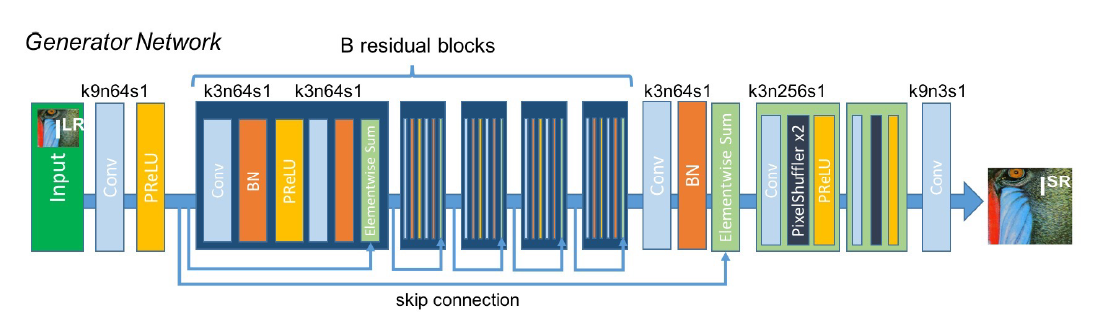
\includegraphics[scale = 0.6]{Imp_generador.png}
    \caption{Arquitectura del generador de la SRGAN,\emph{k} es el tamaño del
    filtro, \emph{n} es la dimensión del mapa de características (capa convolucionada) y \emph{s} indica
    el valor del parámetro stride. Imagen tomada de \cite{SRGAN}}
    \label{Alexis4}
  \end{center}
\end{figure}

\subsubsection{Modelo discriminador.}

\begin{figure}[H]
  \begin{center}
    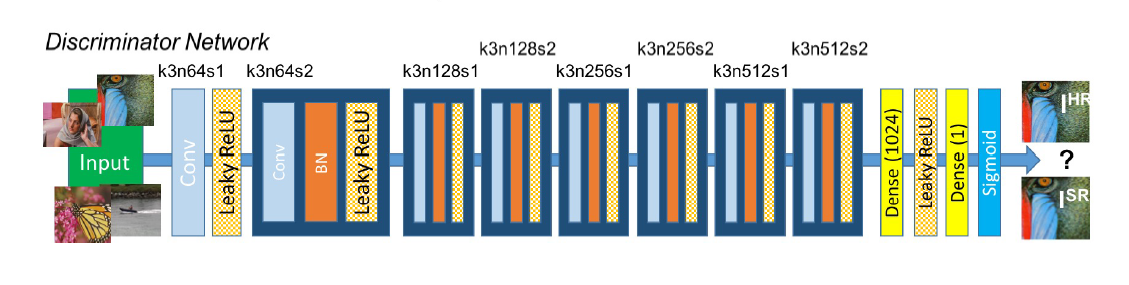
\includegraphics[scale = 0.6]{Imp_discriminador.png}
    \caption{Arquitectura del Discriminador de la SRGAN, \emph{k} es el tamaño
    del filtro, \emph{n} es la dimensión del mapa de características (capa convolucionada) y \emph{s}
    indica el valor del parámetro stride. Imagen tomada de \cite{SRGAN}}
    \label{Alexis5}
  \end{center}
\end{figure}

\subsubsection{Entrenamiento}

EL modelo de entrenamiento de las GAN´s

\begin{figure}[H]
    \begin{center}
      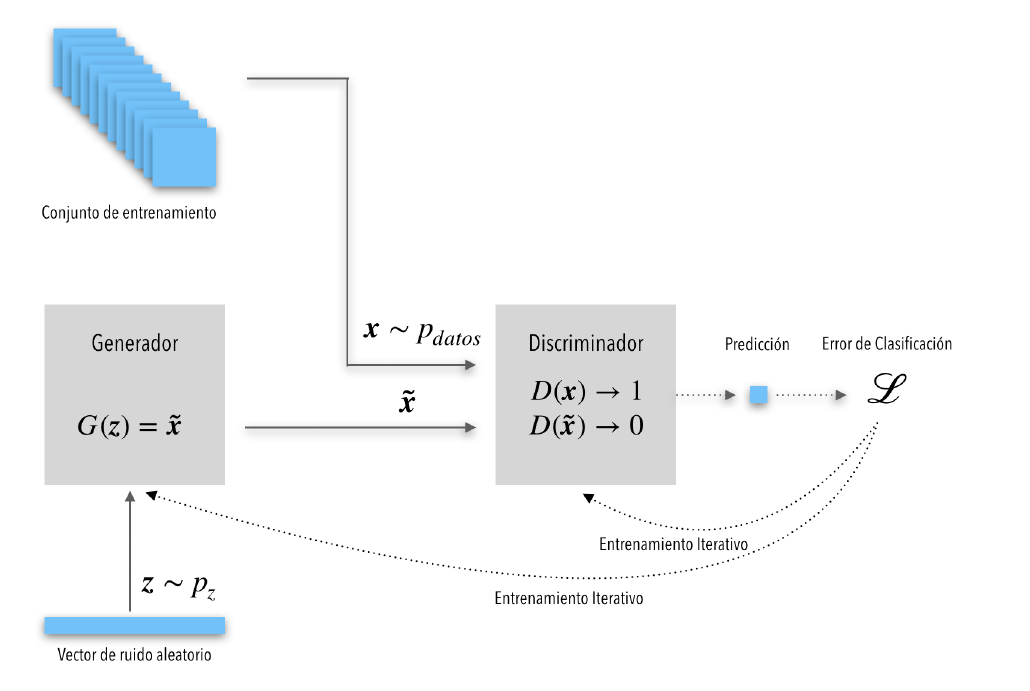
\includegraphics[scale = 0.6]{proceso_gan.png}
      \caption{Proceso de entrenamiento}
      \label{Alexis6}
    \end{center}
\end{figure}

    \section{Resultados}
    \begin{frame}{Resultados (1/3)}

    \begin{figure}[H]
        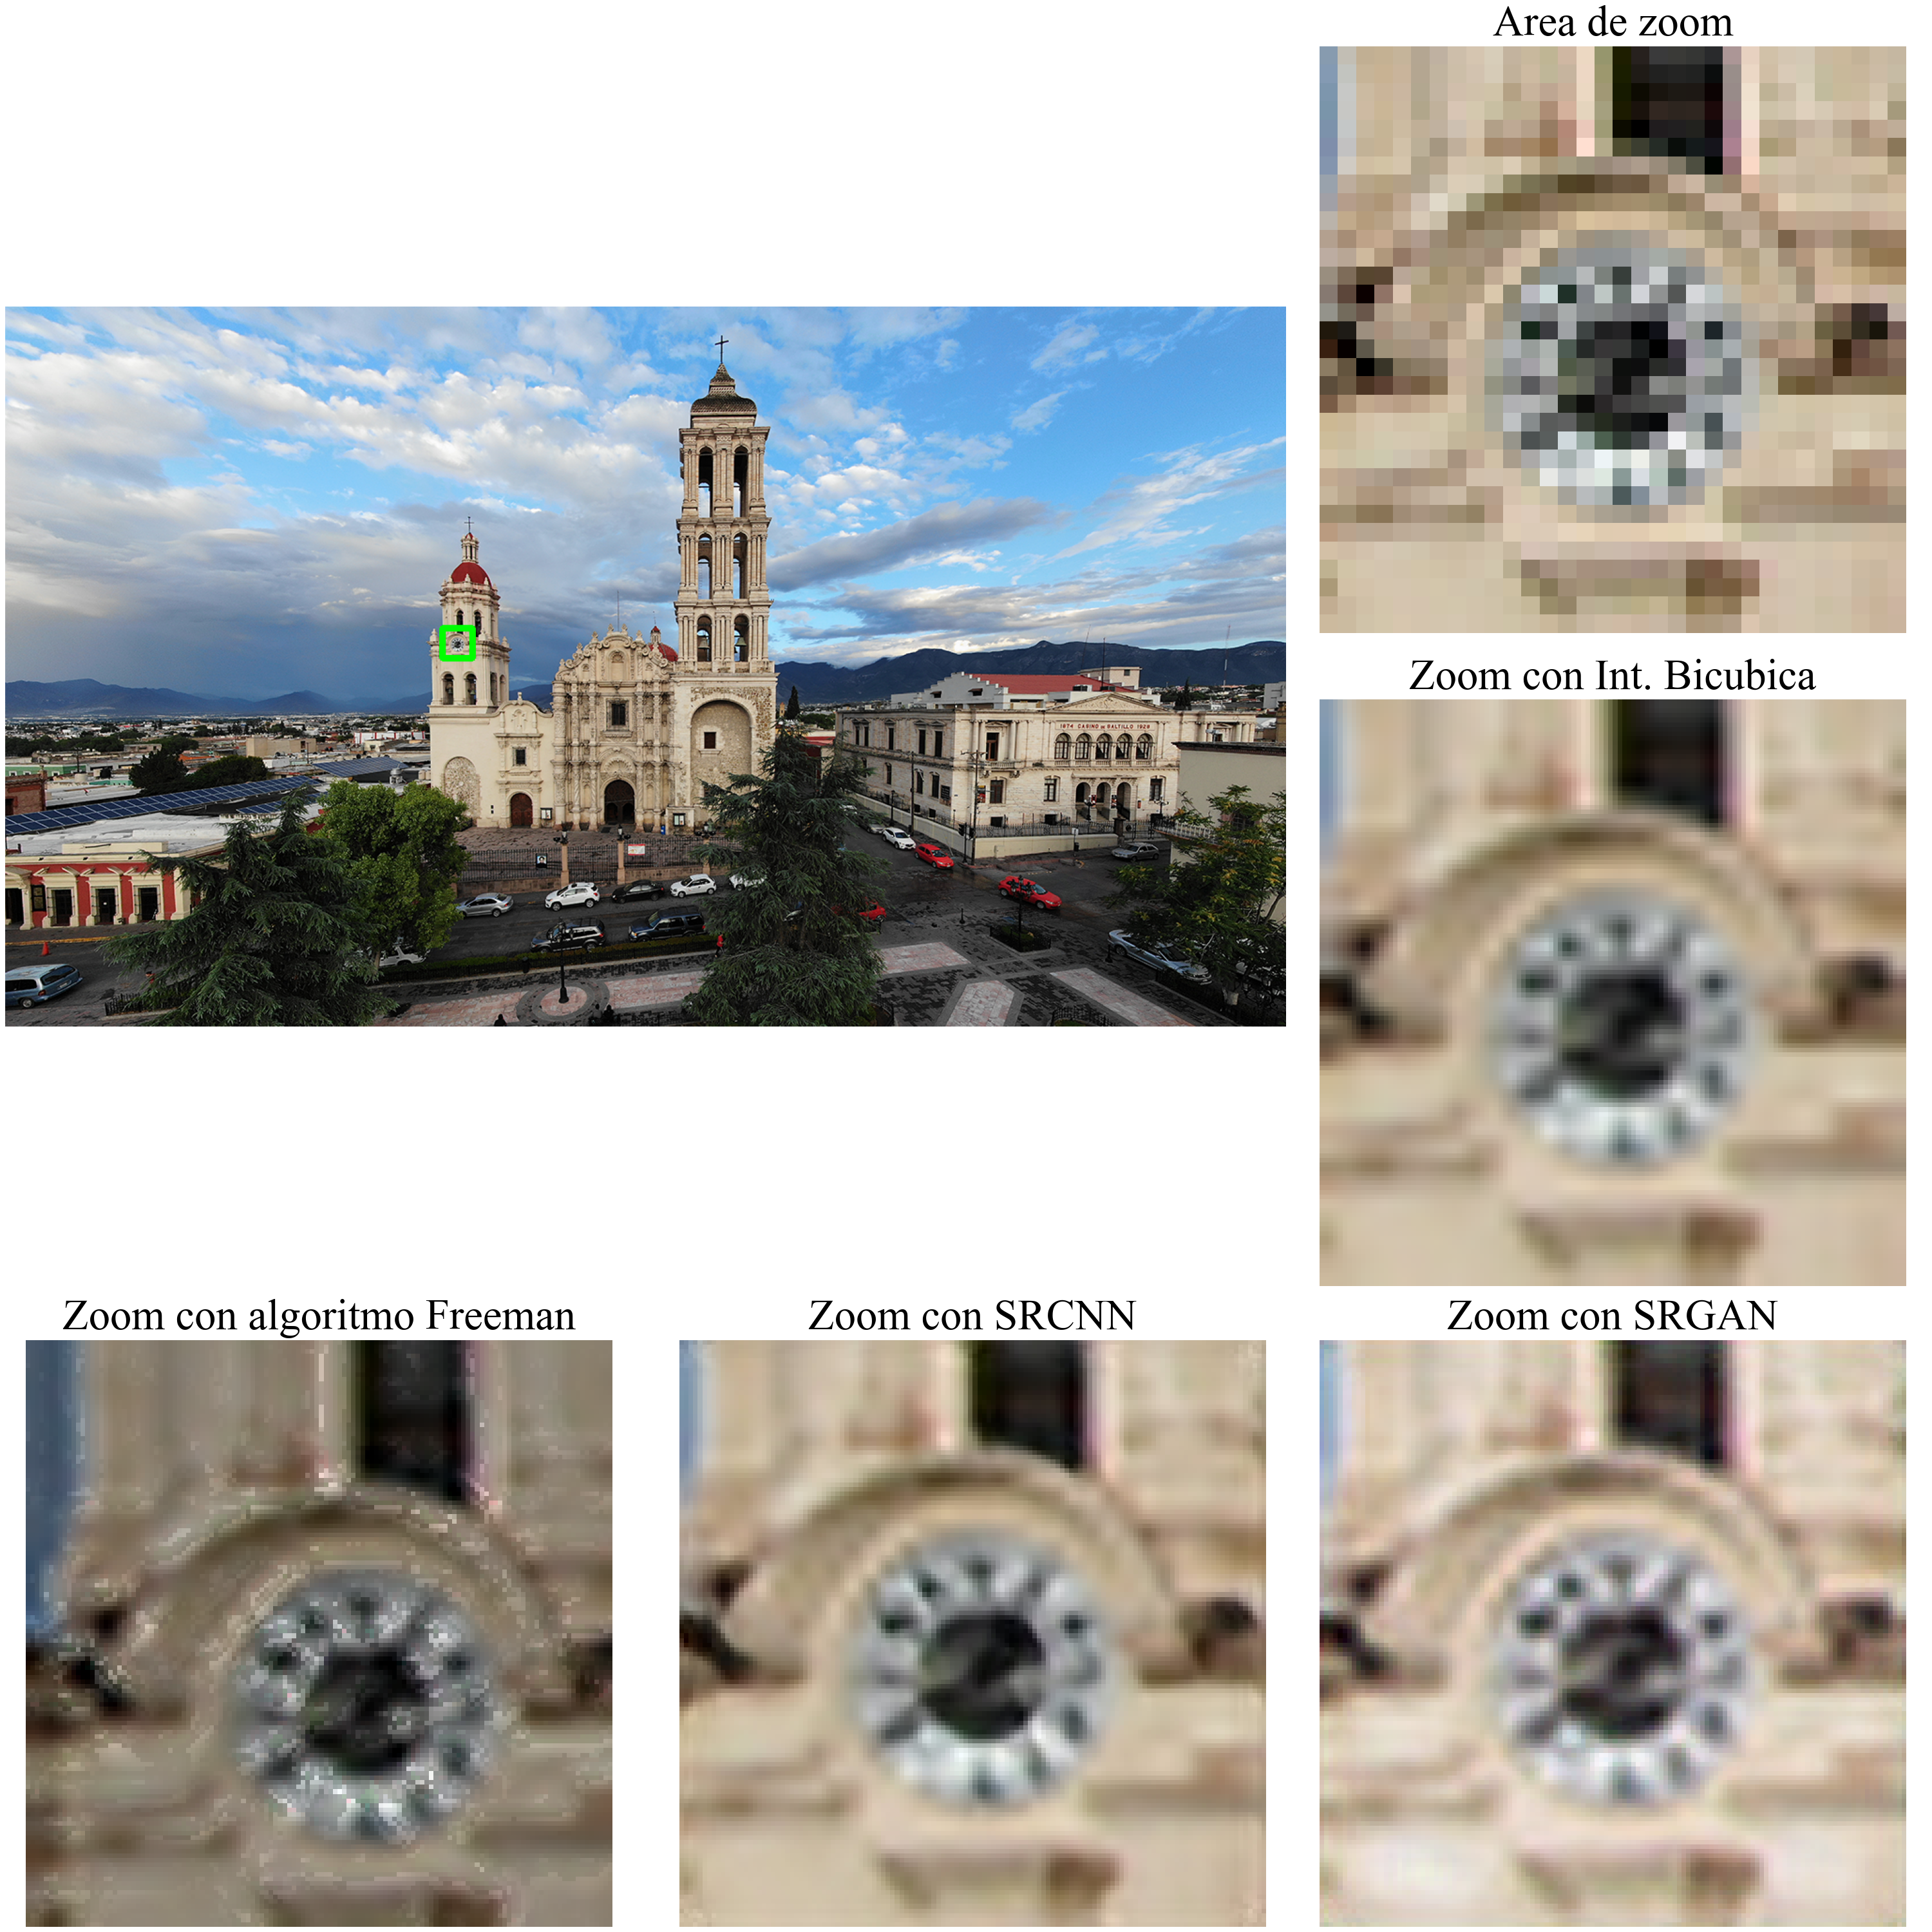
\includegraphics[scale = 0.16]{ ResultadoSaltillo.png}
        \centering
        \caption{Zoom digital en fotografía de Saltillo, Coahuila}
        \label{fig:saltillo}
    \end{figure}

\end{frame}

\begin{frame}{Resultados (2/3)}

    \begin{figure}[H]
        \includegraphics[scale = 0.16]{ ResultadoVilla.png}
        \centering
        \caption{Zoom digital en fotografía de Villahermosa, Tabasco}
        \label{fig:villahermosa}
    \end{figure}
    
\end{frame}

\begin{frame}{Resultados (3/3)}

    \begin{figure}[H]
        \includegraphics[scale = 0.16]{ ResultadoComitan.png}
        \centering
        \caption{Zoom digital en fotografía de Comitán, Chiapas}
        \label{fig:comitan}
    \end{figure}
    
\end{frame}


    \section{Conclusiones}
    \begin{frame}{Conclusiones}
    \begin{block}{}
        \begin{itemize}
            \item La predicción de frecuencias altas resultó útil cuando se 
            requiere mejorar la resolución de una imagen.
            \pause
            \item \emph{SRCNN} y \emph{SRGAN} son más robustas y rápidas en la predicción 
            de la imagen para mejorar su resolución. 
            \pause
            \item El algoritmo de \emph{Freeman et al} tiene una muy buena aproximación
            y su 'entrenamiento' no es tan tardado como los métodos con redes neuronales. 
            \pause
            \item El comportamiento de los tres métodos fue el esperado y representan
            una evolución en tareas de \emph{Súper Resolución}. 
        \end{itemize}
    \end{block}
\end{frame}


    \section{Discusión}
    % Filtros pasa altas para diferentes diccionarios
Para la generación del diccionario del algoritmo de freeman se podría utilizar diferentes filtros pasa altas para obtener otros
diccionarios, de forma que se observen los comportamientos que pueda tener en la generación del parchado de la imagen de
alta resolución.\\
% Factor alfa define el detalle de la imagen a reconstruir pero tambien genera ruido
Se observó que el factor $\alpha$ en el algoritmo de freeman afecta a lo que es el detalle de la imagen, pero a su vez este también genera ruido en la imágen,
por lo que se debe buscar el punto óptimo para este valor, de manera que se balanceen de forma adecuada el detalle de la imagen
así como el ruido que este factor puede generar.\\
% Discusiones de SRCNN
Durante el desarrollo del módelo SRCNN se observó que, cuando se realiza el entrenamiento del módelo para un factor de escalamiento
de \textbf{4}, ya sea en el espacio de color $RGB$ ó $YC_rC_b$ aparentemente se tiene una asintota en $0.003$ de la métrica $MSE$,
y se requeriría realizar un re-entrenamiento de estos modelos para verificar o descartar la existencia de esta asintota. Para
nuestro caso, decidimos detener el entrenamiento de la red en este punto, ya que observamos que la minimización de nuestra función
de coste ($MSE$) era mínima. Lo mismo ocurre para los modelos SRCNN entrenados con un factor de escalamiento de 2 (En ambos
espacios de color), pero en estos módelos, debido a que la imagen de entrenamiento en baja resolución no ha "perdido" tantos
detalles respecto de la imagen original, es que su función de coste $MSE$ se logra reducir en mayor medida, observandose un valor
aparentemente asintótico en $0.0012$, aunque de igual forma que para los modelos con factor de escalamiento 4, habría que re-entrenar
el módelo para verificar esto. Cabe destacar que en este punto para mejorar los módelos es necesario ir ajustando la tasa de aprendizaje
$\alpha$ del optimizador \textbf{Adam} de forma adecuada.\\
Para el módelo entrenado en el espacio de color $YC_rC_b$ se utiliza únicamente el canal $Y$ para el entrenamiento de la red,
esto por que es en este canal en el que se \emph{concentra} la mayor parte de la información de la imagén, ya que si observamos
unicamente este canal por separado el resultado sería la imagen original pero en escala de grises, es por ello que resulta conveniente
este módelo, dado que entrenar la red unicamente sobre un canal hace que la cantidad de parámetros de la red se reduzca, lo cual
puede reducir el tiempo de entrenamiento de la red.


    \Urlmuskip=0mu plus 1mu\relax
    \bibliographystyle{IEEEtran}
    \bibliography{bibliografia}

\end{document}